% =============================================================================
% WEAPON-TARGET ASSIGNMENT PROBLEM - Combined Presentation
% Algorithm Engineering Sessional - Checkpoint Presentation
% =============================================================================

\documentclass[aspectratio=43,8pt]{beamer}

% =============================================================================
% THEME AND COLORS
% =============================================================================
\usetheme{default}
\usecolortheme{default}

% Professional minimal color scheme - muted grayscale
\definecolor{primaryblue}{RGB}{40, 40, 40}
\definecolor{secondaryblue}{RGB}{80, 80, 80}
\definecolor{accentred}{RGB}{100, 100, 100}
\definecolor{accentgreen}{RGB}{60, 60, 60}
\definecolor{lightgray}{RGB}{200, 250, 200}

\setbeamercolor{structure}{fg=primaryblue}
\setbeamercolor{frametitle}{bg=white, fg=primaryblue}
\setbeamercolor{title}{fg=primaryblue}
\setbeamercolor{block title}{bg=lightgray, fg=primaryblue}
\setbeamercolor{block body}{bg=white}
\setbeamercolor{block title alerted}{bg=lightgray, fg=primaryblue}
\setbeamercolor{block title example}{bg=lightgray, fg=primaryblue}

% Simplify itemize bullets
\setbeamertemplate{itemize items}[circle]
\setbeamertemplate{enumerate items}[default]

% Remove shadows and rounded corners for cleaner look
\setbeamertemplate{blocks}[default]
\setbeamertemplate{title page}[default][colsep=-4bp,rounded=false]

% Minimal navigation
\setbeamertemplate{navigation symbols}{}

% Clean frame title with reduced spacing
\setbeamertemplate{frametitle}{
  \vspace{0.2cm}
  \insertframetitle
  \vspace{0.05cm}
  \hrule
  \vspace{0.2cm}
}

% Maximize content area - reduce margins and spacing
\setbeamersize{text margin left=0.5cm,text margin right=0.5cm}
\setlength{\parskip}{3pt}

% =============================================================================
% PACKAGES
% =============================================================================
\usepackage[utf8]{inputenc}
\usepackage[T1]{fontenc}
\usepackage{lmodern}
\usepackage{amsmath}
\usepackage{amssymb}
\usepackage{graphicx}
\usepackage{booktabs}
\usepackage{array}
\usepackage{tikz}
\usetikzlibrary{positioning, arrows.meta, shapes, calc}
\usepackage{algorithm}
\usepackage{algpseudocode}
\usepackage{xcolor}
\usepackage{hyperref}
\usepackage{multirow}

% =============================================================================
% FOOTER CONFIGURATION
% =============================================================================
\setbeamertemplate{navigation symbols}{}
\setbeamertemplate{footline}{
  \hfill\usebeamerfont{page number in head/foot}\insertframenumber{} / \inserttotalframenumber\hspace*{1em}\vskip2pt
}

% =============================================================================
% TITLE INFORMATION
% =============================================================================
\title[WTA Problem]{\textbf{Weapon-Target Assignment Problem}}
\subtitle{Algorithm Engineering Sessional -- Checkpoint Presentation}
\author[Team WTA]{Team Members}
\institute[CSE 462]{CSE 462: Algorithm Engineering Sessional}
\date{January 2026}

% =============================================================================
% DOCUMENT BEGINS
% =============================================================================
\begin{document}

% =============================================================================
% TITLE SLIDE
% =============================================================================
\begin{frame}[plain]
\begin{center}
\vspace{0.3cm}
% BUET Logo

\includegraphics[width=0.15\textwidth]{images/buet_logo.png}

\vspace{0.3cm}
{\Large\textbf{\textcolor{primaryblue}{Weapon-Target Assignment Problem}}}

\vspace{0.3cm}
{\normalsize CSE 462: Algorithm Engineering Sessional}

{\normalsize Checkpoint 1 Presentation}

\vspace{0.5cm}
\begin{tabular}{ll}
\textbf{Team Members} & \\
Hozifa Rahman Hamim & (ID: 1705083) \\
Md. Azizul Haque Nadim & (ID: 1905059) \\
Sadia Tabassum & (ID: 1905091) \\
Ahmmad Nur Swapnil & (ID: 2005009) \\
Most. Sonia Khatun & (ID: 2005025) \\
Shahriar Ahmed Seam & (ID: 2005093) \\
\end{tabular}

\vspace{0.5cm}
{\small Department of Computer Science and Engineering (CSE)}

{\small Bangladesh University of Engineering and Technology (BUET)}

\vspace{0.3cm}
{\footnotesize\textit{19th January 2026}}
\end{center}
\end{frame}

% =============================================================================
% REAL-WORLD WTA EXAMPLES SLIDE
% =============================================================================
\begin{frame}{Real-World Motivation: WTA in Action}
\begin{columns}[t]
\column{0.48\textwidth}
\begin{center}
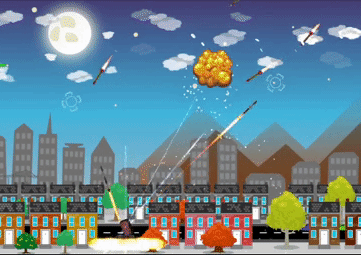
\includegraphics[width=0.95\textwidth]{images/iron_dome_image.png}

{\footnotesize\textbf{Air Defense (Iron Dome)}}
\end{center}

\vspace{0.1cm}
{\scriptsize\textbf{WTA Mapping:}}
\begin{itemize}\setlength{\itemsep}{0pt}
    \item[\textcolor{blue}{$\bullet$}] Interceptor Missiles = \textbf{Weapons}
    \item[\textcolor{red}{$\bullet$}] Incoming Rockets = \textbf{Targets}
    \item[\textcolor{green!60!black}{$\rightarrow$}] Assignment = \textbf{WTA Solution}
\end{itemize}

\column{0.52\textwidth}
\begin{center}
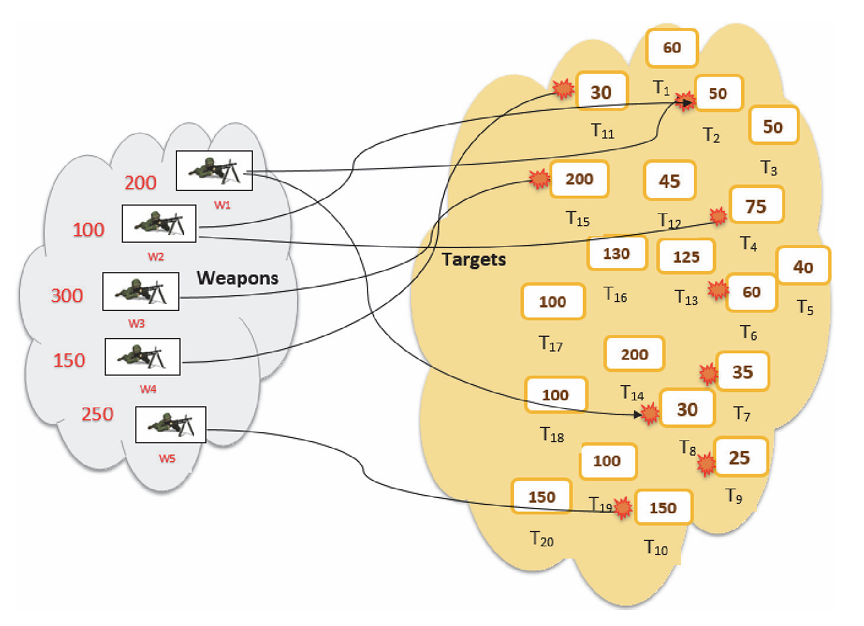
\includegraphics[width=0.95\textwidth]{images/ground_attack_image.png}

{\footnotesize\textbf{Ground Attack Scenario}}
\end{center}

\vspace{0.1cm}
{\scriptsize\textbf{WTA Mapping:}}
\begin{itemize}\setlength{\itemsep}{0pt}
    \item[\textcolor{blue}{$\bullet$}] W1--W5 (with costs) = \textbf{Weapons}
    \item[\textcolor{red}{$\bullet$}] T1--T20 (with values) = \textbf{Targets}
    \item[\textcolor{green!60!black}{$\rightarrow$}] Arrows = \textbf{Assignments}
\end{itemize}
\end{columns}
\end{frame}

% =============================================================================
% OUTLINE SLIDE
% =============================================================================
\begin{frame}{Presentation Outline}
\begin{columns}[t]
\column{0.48\textwidth}
\begin{block}{Part 1: Theory}
\begin{enumerate}
    \item \textbf{Problem Definition}
    \begin{itemize}
        \item Formal definition
        \item Mathematical formulation
        \item Classifications
    \end{itemize}
    \item \textbf{NP-Hardness Proofs}
    \begin{itemize}
        \item Reduction from SUBSET PRODUCT
        \item Reduction to Multiple Knapsack
    \end{itemize}
    \item \textbf{Algorithm Survey}
    \begin{itemize}
        \item Exact, approximation, heuristic algorithms
    \end{itemize}
\end{enumerate}
\end{block}

\column{0.48\textwidth}
\begin{block}{Part 2: Implementation}
\begin{enumerate}
\setcounter{enumi}{3}
    \item \textbf{Selected Algorithms}
    \begin{itemize}
        \item Maximum Marginal Return (MMR)
        \item Ant Colony Optimization (ACO)
    \end{itemize}
    \item \textbf{Experimental Design}
    \begin{itemize}
        \item Benchmark instances
        \item Metrics and analysis plan
    \end{itemize}
    \item \textbf{Applications}
    \begin{itemize}
        \item Military and civilian uses
    \end{itemize}
\end{enumerate}
\end{block}
\end{columns}

% \vspace{0.3cm}
% \begin{center}
% \textcolor{gray}{\footnotesize Total Time: 15 minutes (6 sections $\times$ 2.5 minutes each)}
% \end{center}
\end{frame}

% =============================================================================
% SECTION 1: PROBLEM DEFINITION
% =============================================================================
\section{Problem Definition}

\begin{frame}{Section 1: Problem Definition}
\begin{center}
{\Large\textcolor{primaryblue}{\textbf{What is the Weapon-Target Assignment Problem?}}}

\vspace{0.5cm}
{\normalsize A fundamental combinatorial optimization problem in operations research}
\end{center}
\end{frame}

\begin{frame}{Problem Definition}
\begin{block}{Weapon-Target Assignment (WTA) Problem}
The WTA problem involves the \textbf{strategic allocation of a set of weapons to a set of targets} to achieve a specific defensive or offensive objective.
\end{block}

\vspace{0.3cm}
\begin{alertblock}{Core Challenge: Stochastic Nature of Combat}
Every engagement is modeled as a \textbf{probabilistic event} where a weapon has a specific likelihood of destroying its assigned target.
\end{alertblock}

\vspace{0.3cm}
\begin{exampleblock}{Computational Complexity}
\begin{itemize}
    \item The problem is mathematically proven to be \textbf{NP-complete}
    \item As the number of weapons and targets grows, complexity increases \textbf{exponentially}
    \item Finding an absolute optimal solution becomes extremely difficult for large instances
\end{itemize}
\end{exampleblock}
\end{frame}

\begin{frame}{Classification: Asset-based vs. Target-based}
\begin{block}{Two Perspectives of WTA}
The WTA problem can be viewed from two distinct perspectives depending on whether the objective prioritizes \textbf{destruction of enemy forces} or \textbf{protection of friendly resources}.
\end{block}

\vspace{0.3cm}
\begin{columns}[t]
\column{0.48\textwidth}
\begin{alertblock}{Target-based Perspective}
Values assigned to each \textbf{enemy target} based on threat they pose.
\begin{itemize}
    \item \textbf{Goal:} Maximize total damage inflicted on incoming targets
    \item \textbf{Math:} \textbf{Minimize} expected survival value of targets
    \item (Equivalent to maximizing damage)
\end{itemize}
\end{alertblock}

\column{0.48\textwidth}
\begin{exampleblock}{Asset-based Perspective}
Values assigned to \textbf{defended assets} (cities, bases) rather than targets.
\begin{itemize}
    \item \textbf{Goal:} Maximize combined survival value of friendly assets
    \item \textbf{Requirement:} Map which targets attack which assets
    \item \textbf{Math:} \textbf{Maximize} expected value of surviving assets
\end{itemize}
\end{exampleblock}
\end{columns}
\end{frame}

\begin{frame}{Mathematical Representation: Parameters and Variables}
\begin{block}{Target-based Formulation -- Parameters}
\begin{itemize}
    \item $W = \{1, \dots, m\}$: The set of available \textbf{weapon types}
    \item $T = \{1, \dots, n\}$: The set of \textbf{targets} to be engaged
    \item $v_j$: The \textbf{strategic military value} or importance of target $j$
    \item $p_{ij}$: The ``\textbf{probability of kill}'' -- chance that one weapon of type $i$ will destroy target $j$
    \item $w_i$: The \textbf{total quantity} of weapons of type $i$ available
\end{itemize}
\end{block}

\vspace{0.3cm}
\begin{exampleblock}{Decision Variable}
$$x_{ij} \in \{0, 1, 2, \dots\}$$
\textbf{Integer variable} representing the number of weapons of type $i$ assigned to target $j$
\end{exampleblock}
\end{frame}

\begin{frame}{Mathematical Representation: Objective Functions}
\begin{block}{Goal: Maximize damage (or equivalently, minimize survival)}
While the goal is to maximize damage, the standard convention is to minimize remaining survival value.
\end{block}

\vspace{0.2cm}
\begin{columns}[t]
\column{0.48\textwidth}
\begin{alertblock}{1. Maximizing Total Expected Damage}
\begin{equation*}
\text{Max } Z = \sum_{j=1}^{n} v_j \left[ 1 - \prod_{i=1}^{m} (1 - p_{ij})^{x_{ij}} \right]
\end{equation*}
\end{alertblock}

\column{0.48\textwidth}
\begin{exampleblock}{2. Minimizing Expected Survival Value}
\begin{equation*}
\text{Min } Z = \sum_{j=1}^{n} v_j \prod_{i=1}^{m} (1 - p_{ij})^{x_{ij}}
\end{equation*}
\end{exampleblock}
\end{columns}

\vspace{0.3cm}
\begin{block}{Key Insight}
$\prod_{i=1}^{m} (1 - p_{ij})^{x_{ij}}$ = \textbf{Probability that target $j$ survives ALL assigned weapons}

The product captures the \textbf{combined effect} of multiple weapons attacking the same target.
\end{block}
\end{frame}

\begin{frame}{Mathematical Representation: Constraints}
\begin{block}{Constraint 1: Resource Availability}
\begin{equation*}
\sum_{j=1}^{n} x_{ij} \le w_i, \quad \forall i \in W
\end{equation*}
\textbf{Meaning:} Total weapons of type $i$ assigned across all targets cannot exceed available quantity $w_i$
\end{block}

\vspace{0.3cm}
\begin{alertblock}{Constraint 2: Integrality}
\begin{equation*}
x_{ij} \in \{0, 1, 2, \dots\}
\end{equation*}
\textbf{Meaning:} We can only assign \textbf{whole numbers} of weapons (discrete assignments)
\end{alertblock}

\vspace{0.3cm}
\begin{exampleblock}{Complete Formulation Summary}
\textbf{Minimize} $\sum_{j} v_j \prod_{i} (1-p_{ij})^{x_{ij}}$ \quad
\textbf{s.t.} $\sum_{j} x_{ij} \le w_i$, \quad $x_{ij} \in \mathbb{Z}^+$
\end{exampleblock}
\end{frame}

\begin{frame}{Linear vs. Non-Linear Assignment}
\begin{columns}[t]
\column{0.48\textwidth}
\begin{block}{Linear Assignment Problem (LAP)}
\begin{itemize}
    \item \textbf{Structure:} One weapon assigned to exactly one target (\textbf{One-to-One})
    \item \textbf{Linearity:} Objective function is linear
    \item Assignments are \textbf{independent}
    \item \textcolor{accentgreen}{\textbf{Polynomial time solvable}} (Hungarian algorithm)
\end{itemize}
\end{block}

\column{0.48\textwidth}
\begin{alertblock}{Non-Linear Assignment (Non-LAP)}
\begin{itemize}
    \item \textbf{Structure:} Multiple weapons can be assigned to single target (\textbf{Many-to-One})
    \item \textbf{Non-Linearity:} Due to ``\textbf{diminishing returns}''
    \item Additional weapons = \textbf{overkill} effect
    \item \textcolor{accentred}{\textbf{NP-complete!}}
\end{itemize}
\end{alertblock}
\end{columns}

\vspace{0.3cm}
\begin{center}
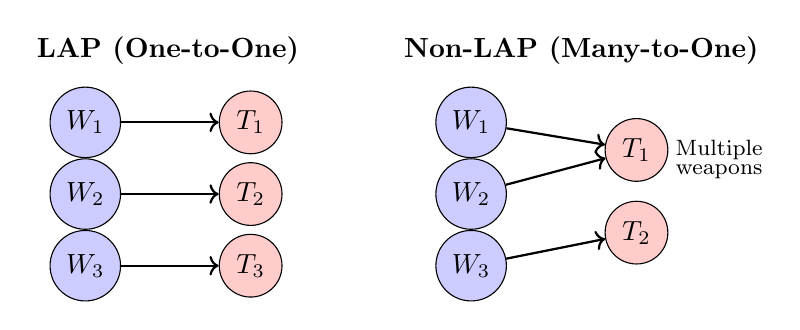
\begin{tikzpicture}[scale=0.7]
% LAP
\node at (-3.5, 1.8) {\textbf{LAP (One-to-One)}};
\node[circle, draw, fill=blue!20, minimum size=0.6cm] (w1) at (-5, 0.5) {$W_1$};
\node[circle, draw, fill=blue!20, minimum size=0.6cm] (w2) at (-5, -0.8) {$W_2$};
\node[circle, draw, fill=blue!20, minimum size=0.6cm] (w2b) at (-5, -2.1) {$W_3$};
\node[circle, draw, fill=red!20, minimum size=0.6cm] (t1) at (-2, 0.5) {$T_1$};
\node[circle, draw, fill=red!20, minimum size=0.6cm] (t2) at (-2, -0.8) {$T_2$};
\node[circle, draw, fill=red!20, minimum size=0.6cm] (t2b) at (-2, -2.1) {$T_3$};
\draw[->, thick] (w1) -- (t1);
\draw[->, thick] (w2) -- (t2);
\draw[->, thick] (w2b) -- (t2b);

% Non-LAP
\node at (4, 1.8) {\textbf{Non-LAP (Many-to-One)}};
\node[circle, draw, fill=blue!20, minimum size=0.6cm] (w3) at (2, 0.5) {$W_1$};
\node[circle, draw, fill=blue!20, minimum size=0.6cm] (w4) at (2, -0.8) {$W_2$};
\node[circle, draw, fill=blue!20, minimum size=0.6cm] (w5) at (2, -2.1) {$W_3$};
\node[circle, draw, fill=red!20, minimum size=0.6cm] (t3) at (5, 0) {$T_1$};
\node[circle, draw, fill=red!20, minimum size=0.6cm] (t4) at (5, -1.5) {$T_2$};
\draw[->, thick] (w3) -- (t3);
\draw[->, thick] (w4) -- (t3);
\draw[->, thick] (w5) -- (t4);
\node at (6.5, 0) {\footnotesize Multiple};
\node at (6.5, -0.4) {\footnotesize weapons};
\end{tikzpicture}
\end{center}
\end{frame}

% =============================================================================
% SECTION 2: NP-HARDNESS PROOFS
% =============================================================================
\section{NP-Hardness Proofs}

\begin{frame}{Section 2: NP-Hardness Proofs}
\begin{center}
{\Large\textcolor{primaryblue}{\textbf{Polynomial-Time Reductions}}}

\vspace{0.5cm}
{\normalsize Proving WTA is NP-complete through formal reductions}
\end{center}
\end{frame}

\begin{frame}{WTA Decision Problem}
\begin{block}{Decision Version of WTA}
\textbf{Given:}
\begin{itemize}
    \item Survival probability $q_{i,j} = 1 - p_{i,j}$
    \item Threshold value $k$
\end{itemize}

\textbf{Question:} Does there exist an assignment $x_{i,j} \in \{0,1\}$ such that:
\begin{equation*}
D = \sum_{j=1}^n V_j \prod_{i=1}^m q_{i,j}^{x_{i,j}} \leq k
\end{equation*}
\end{block}

\begin{alertblock}{Subject to Constraints}
$$\sum_{j=1}^n x_{i,j} \leq W_i \quad \text{for } i = 1, \ldots, m$$
$$x_{i,j} \in \{0, 1\}$$
where $x_{i,j} = 1$ if weapon $i$ assigned to target $j$, and $x_{i,j} = 0$ otherwise.

$D$ represents \textbf{total expected damage} (weighted survival probability of all targets)
\end{alertblock}
\end{frame}

\begin{frame}{Two Polynomial-Time Reductions}
\begin{block}{Our Approach}
We demonstrate two polynomial-time reductions:
\end{block}

\vspace{0.3cm}
\begin{columns}[t]
\column{0.48\textwidth}
\begin{alertblock}{Reduction 1}
\textbf{SUBSET PRODUCT $\leq_p$ WTA}

\vspace{0.2cm}
$\Rightarrow$ Proves \textbf{WTA is NP-hard}

\vspace{0.2cm}
{\small (Reduce FROM a known NP-complete problem TO WTA)}
\end{alertblock}

\column{0.48\textwidth}
\begin{exampleblock}{Reduction 2}
\textbf{WTA $\leq_p$ Multiple Knapsack}

\vspace{0.2cm}
$\Rightarrow$ Shows WTA reduces to another known NP-hard problem

\vspace{0.2cm}
{\small (Shows connection between problems)}
\end{exampleblock}
\end{columns}

\vspace{0.5cm}
\begin{center}
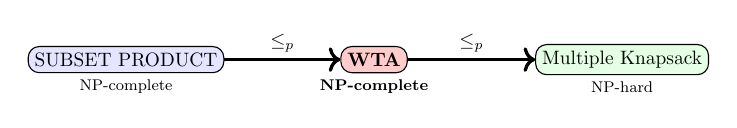
\begin{tikzpicture}[scale=0.7, transform shape]
\node[draw, rounded corners, fill=blue!10] (sp) at (0,0) {SUBSET PRODUCT};
\node[draw, rounded corners, fill=red!20] (wta) at (4.5,0) {\textbf{WTA}};
\node[draw, rounded corners, fill=green!10] (mk) at (9,0) {Multiple Knapsack};
\draw[->, very thick] (sp) -- node[above] {$\leq_p$} (wta);
\draw[->, very thick] (wta) -- node[above] {$\leq_p$} (mk);
\node[below] at (sp.south) {\footnotesize NP-complete};
\node[below] at (wta.south) {\footnotesize \textbf{NP-complete}};
\node[below] at (mk.south) {\footnotesize NP-hard};
\end{tikzpicture}
\end{center}
\end{frame}

\begin{frame}{Reduction 1: SUBSET PRODUCT $\leq_p$ WTA}
\begin{block}{SUBSET PRODUCT Problem (NP-complete)}
\textbf{Given:} Set $A = \{a_1, a_2, \ldots, a_m\}$ and target product $b$

\textbf{Find:} Subset $X \subseteq A$ where $\prod_{x \in X} a_x = b$
\end{block}

\vspace{0.2cm}
\begin{exampleblock}{WTA Instance Construction}
Let $P = \prod_{i=1}^m a_i$. Construct WTA with:
\begin{itemize}
    \item \textbf{Targets:} 2 targets with values $V_1 = V_2 = P$
    \item \textbf{Weapons:} $m + 2$ weapons: $W_1, W_2, \ldots, W_m, W_\alpha, W_\beta$
    \item \textbf{Survival probabilities:}
    \begin{columns}
    \column{0.45\textwidth}
    \begin{itemize}
        \item $q_{i,1} = q_{i,2} = \frac{1}{a_i}$ for $i = 1, \ldots, m$
    \end{itemize}
    \column{0.45\textwidth}
    \begin{itemize}
        \item $q_{\alpha,1} = q_{\alpha,2} = \frac{b}{2P}$
        \item $q_{\beta,1} = q_{\beta,2} = \frac{1}{2b}$
    \end{itemize}
    \end{columns}
    \item \textbf{Threshold:} $k = 1$ (we ask if $D \leq 1$)
\end{itemize}
\end{exampleblock}

\begin{alertblock}{Time Complexity}
Constructs WTA with 2 targets and $m+2$ weapons in $O(m)$ time -- \textbf{Polynomial!}
\end{alertblock}
\end{frame}

\begin{frame}{Reduction 1: Forward Direction}
\begin{block}{Forward ($\Rightarrow$): SUBSET PRODUCT has solution $\Rightarrow$ WTA has solution}
Suppose $X \subseteq \{1, \ldots, m\}$ with $\prod_{x \in X} a_x = b$. Let $Y = \{1, \ldots, m\} \setminus X$.

Then:
$$\prod_{i \in X} \frac{1}{a_i} = \frac{1}{b}, \quad \prod_{y \in Y} \frac{1}{a_y} = \frac{b}{P}$$

\textbf{Assignment:} $\{W_x : x \in X\} \cup \{W_\alpha\} \rightarrow T_1$ and $\{W_y : y \in Y\} \cup \{W_\beta\} \rightarrow T_2$

\textbf{Total damage:}
\begin{align*}
D &= V_1 \cdot \frac{b}{2P} \cdot \frac{1}{b} + V_2 \cdot \frac{1}{2b} \cdot \frac{b}{P} \\
&= P \cdot \frac{b}{2P} \cdot \frac{1}{b} + P \cdot \frac{1}{2b} \cdot \frac{b}{P} = \frac{1}{2} + \frac{1}{2} = 1 \leq k \quad \checkmark
\end{align*}
\end{block}
\end{frame}

\begin{frame}{Reduction 1: Backward Direction (Part 1)}
\begin{block}{Backward ($\Leftarrow$): WTA has solution $\Rightarrow$ SUBSET PRODUCT has solution}
Suppose WTA has solution with $D \leq 1$. Let $X', Y'$ be weapons assigned to $T_1, T_2$.
\end{block}

\begin{alertblock}{Claim: $W_\alpha$ and $W_\beta$ cannot both target the same target}
\textit{Proof:} If both assigned to $T_1$ (symmetric for $T_2$):
$$D \geq P \cdot \frac{1}{2b} \cdot \frac{b}{2P} \cdot \frac{1}{\prod_{x \in X' \setminus \{\alpha, \beta\}} a_x} + \frac{P}{\prod_{y \in Y'} a_y} \geq \frac{1}{4} + 1 > 1 \quad \Rightarrow\!\Leftarrow$$

So $W_\alpha \to T_1$ and $W_\beta \to T_2$. Let $X = X' \setminus \{\alpha\}$, $Y = Y' \setminus \{\beta\}$.
\end{alertblock}

\begin{block}{From the Assignment}
With $W_\alpha \to T_1$ and $W_\beta \to T_2$:
$$D = P \cdot \frac{b}{2P} \prod_{x \in X} \frac{1}{a_x} + P \cdot \frac{1}{2b} \prod_{y \in Y} \frac{1}{a_y} \leq 1$$
\end{block}

\end{frame}

\begin{frame}{Reduction 1: Backward Direction (Part 2)}

\begin{exampleblock}{Algebraic Derivation}
Let $z = \prod_{x \in X} a_x$. Then:
$$\frac{b}{2z} + \frac{z}{2b} \leq 1$$

Multiply by $2bz > 0$:
$$b^2 + z^2 \leq 2bz \quad \Rightarrow \quad (b - z)^2 \leq 0$$

Since $(b-z)^2 \geq 0$, we must have $(b-z)^2 = 0$, so:
$$b = z = \prod_{x \in X} a_x$$
\end{exampleblock}

\begin{alertblock}{Conclusion}
$X$ is a valid solution to SUBSET PRODUCT! $\checkmark$

\textbf{Time Complexity:} $O(m)$ -- Polynomial reduction complete.
\end{alertblock}
\end{frame}

\begin{frame}{Reduction 2: WTA $\leq_p$ Multiple Knapsack}
\begin{block}{Multiple Knapsack Construction}
Given WTA with $m$ targets, $n$ weapons, probabilities $\{p_{i,j}\}$:
\begin{itemize}
    \item \textbf{Knapsacks:} $m$ knapsacks (one per target) with Capacity $C_j = \infty$
    % \item \textbf{Capacity:} $C_j = \infty$ (or sufficiently large)
    \item \textbf{Items:} $w_i$ items for weapon type $i$ (one per copy)
    \item \textbf{Profit:} $v_{ij} = -\log(1 - p_{i,j}) = -\log(q_{i,j})$
    \item \textbf{Question:} Does assignment with value $\geq V$ exist?
\end{itemize}
\end{block}

\begin{exampleblock}{Objective Transformation (Key Insight)}
For single target $j$, minimizing $\prod q_{i,j}^{x_{i,j}}$ equals minimizing:
$$\log\left(\prod_{i=1}^n q_{i,j}^{x_{i,j}}\right) = \sum_{i=1}^n x_{i,j} \log(q_{i,j})$$

Equivalent to \textbf{maximizing}:
$$-\sum_{i=1}^n x_{i,j} \log(q_{i,j}) = \sum_{i=1}^n x_{i,j} \cdot v_{ij}$$

This is \textbf{exactly the Multiple Knapsack objective!}
\end{exampleblock}
\end{frame}

\begin{frame}{Reduction 2: Constraint Mapping \& Conclusion}

\begin{block}{Constraint Mapping}
\begin{itemize}
    \item \textbf{WTA constraint:} $\sum_{j=1}^m x_{i,j} \leq W_i$ (weapon type $i$ used at most $W_i$ times)
    \item \textbf{Maps to:} $\sum_{j=1}^m y_{ij} \leq 1$ (each item in at most one knapsack) when $W_i = 1$
    \item For general $W_i$: Create $W_i$ copies of item $i$
\end{itemize}
\end{block}

\begin{exampleblock}{Equivalence}
Assignment $x_{i,j}$ optimal for WTA $\Leftrightarrow$ $y_{ij} = x_{i,j}$ optimal for Multiple Knapsack

\textbf{Logarithmic transformation preserves ordering of solutions!}

\textbf{Time:} $O(nm)$ to compute all $v_{ij} = -\log(1 - p_{i,j})$
\end{exampleblock}

\begin{alertblock}{Final Conclusion}
\begin{center}
\textbf{WTA is in NP} (solution verifiable in polynomial time) + \textbf{WTA is NP-hard}

$\Rightarrow$ \textbf{The Weapon-Target Assignment Problem is NP-complete!}
\end{center}
\end{alertblock}
\end{frame}

% =============================================================================
% SECTION 3: ALGORITHM TABLE
% =============================================================================
\section{Algorithm Survey}

\begin{frame}{Section 3: Existing Algorithms Survey}
\begin{center}
{\Large\textcolor{primaryblue}{\textbf{Comprehensive Algorithm Categories for WTA}}}

\vspace{0.5cm}
{\normalsize Five major categories of solution approaches}
\end{center}

\vspace{0.3cm}
\begin{columns}[t]
\column{0.32\textwidth}
\begin{block}{Exact}
\begin{itemize}
    \item Optimal solutions
    \item Exponential time
    \item Small instances
\end{itemize}
\end{block}

\column{0.32\textwidth}
\begin{alertblock}{Approximation}
\begin{itemize}
    \item Provable bounds
    \item Polynomial time
    \item Large instances
\end{itemize}
\end{alertblock}

\column{0.32\textwidth}
\begin{exampleblock}{Randomized}
\begin{itemize}
    \item Probabilistic
    \item Quality $\propto$ samples
    \item Baseline approach
\end{itemize}
\end{exampleblock}
\end{columns}

\vspace{0.3cm}
\begin{columns}[c]
\column{0.45\textwidth}
\begin{block}{Heuristic}
Fast, problem-specific, near-optimal
\end{block}

\column{0.45\textwidth}
\begin{alertblock}{Metaheuristic}
General-purpose, exploration/exploitation balance
\end{alertblock}
\end{columns}
\end{frame}

\begin{frame}{Category 1: Exact Exponential Algorithms}
\begin{block}{Guarantee Optimal Solutions with Proven Bounds}
These algorithms guarantee finding the optimal solution but have exponential time complexity.
\end{block}

\vspace{0.2cm}
\begin{table}[h]
\centering
\small
\begin{tabular}{p{1.8cm}p{3.8cm}p{1.6cm}p{1.7cm}p{0.6cm}}
\toprule
\textbf{Algorithm} & \textbf{Description} & \textbf{Complexity} & \textbf{Solution Quality} & \textbf{Ref} \\
\midrule
\textbf{Branch-and-Bound (B\&B)} & Uses LP/IP relaxations with branching on weapon-target assignments. Employs maximum marginal return for branching strategy and network flow for lower bounds. & Worst-case: $O(2^{mn})$ nodes & \textcolor{accentgreen}{Optimal}; handles up to $80 \times 80$ instances & \cite{ahuja2007} \\
\addlinespace
\textbf{Branch-Price-and-Cut (BPC)} & Reformulates WTA for column generation with efficient pricing problem solver. Uses clique cuts and power cone optimization for tight relaxations. & Polynomial per iteration; $O(nm \cdot K)$ & \textcolor{accentgreen}{Optimal}; solves $10000+$ in seconds & \cite{bertsimas2025} \\
\addlinespace
\textbf{Branch-and-Adjust} & Specialized B\&B using compact piecewise linear convex under-approximation of objective. Built on MILP solvers with custom callbacks. & Exponential worst; poly approx & \textcolor{accentgreen}{Optimal}; 2\% gap for $1500 \times 1000$ in 2h & \cite{andersen2022} \\
\bottomrule
\end{tabular}
\end{table}

\end{frame}

\begin{frame}{Category 2: Approximation Algorithms}
\begin{block}{Provable Bounds with Polynomial Time Complexity}
These algorithms provide theoretical guarantees on solution quality while running in polynomial time.
\end{block}

\vspace{0.2cm}
\begin{table}[h]
\centering
\small
\begin{tabular}{p{1.8cm}p{3.6cm}p{1.6cm}p{1.7cm}p{0.8cm}}
\toprule
\textbf{Algorithm} & \textbf{Description} & \textbf{Complexity} & \textbf{Solution Quality} & \textbf{Ref} \\
\midrule
\textbf{Piecewise Linear Approximation} & Approximates nonlinear survival probability using piecewise linear convex functions with breakpoints. Based on logarithmic transformation $-\log(1-p_{ij})$. & $O(mn \cdot B)$ where $B$ = breakpoints & Provable $\delta$-error bounds; suboptimal but efficient & \cite{camm2002,andersen2022} \\
\addlinespace
\textbf{LP Relaxation + Rounding} & Relaxes integer constraints to LP, solves continuous problem, then rounds to feasible integer solution using various rounding schemes. & $O(\text{poly}(m,n))$ (interior point) & No approximation guarantee; may violate constraints & \cite{ahuja2007} \\
\addlinespace
\textbf{Lagrangian Relaxation} & Relaxes weapon constraints via Lagrangian multipliers, decomposes into independent target subproblems. Uses subgradient method for multiplier updates. & $O(T \cdot nm)$ where $T$ = iterations & Provides lower bounds; typically \textcolor{orange}{5-15\%} gap & \cite{kwon1999,kim2022} \\
\bottomrule
\end{tabular}
\end{table}

\end{frame}

\begin{frame}{Category 3: Randomized Algorithms}
\begin{block}{Probabilistic Methods for Solution Space Exploration}
These algorithms use randomness to explore the solution space.
\end{block}

\vspace{0.3cm}
\begin{table}[h]
\centering
\small
\begin{tabular}{p{1.8cm}p{3.6cm}p{1.6cm}p{1.7cm}p{0.8cm}}
\toprule
\textbf{Algorithm} & \textbf{Description} & \textbf{Complexity} & \textbf{Solution Quality} & \textbf{Ref} \\
\midrule
\textbf{Monte Carlo Sampling} & Generates multiple random weapon-target assignments, evaluates each using survival probability function, selects best assignment. & $O(S \cdot mn)$ where $S$ = samples & Baseline; expected value $\to$ optimal as $S \to \infty$ & \cite{hindawi2017} \\
\addlinespace
\textbf{Randomized Constructive Heuristic} & Builds solutions by probabilistically selecting weapon-target pairs based on marginal returns with added randomness to escape local optima. & $O(R \cdot mn)$ where $R$ = restarts & Variable $(\pm 10\text{-}20\%)$; depends on random seed & \cite{kline2020} \\
\bottomrule
\end{tabular}
\end{table}

% \vspace{0.3cm}
% \begin{alertblock}{Key Insight}
% Randomized algorithms are useful as \textbf{baselines} and for generating \textbf{diverse initial solutions} for other methods.
% \end{alertblock}
\end{frame}

\begin{frame}{Category 4: Heuristic Algorithms}
\begin{block}{Problem-Specific Knowledge for Fast Good Solutions}
Heuristics use domain knowledge to quickly find good (but not necessarily optimal) solutions.
\end{block}

\vspace{0.2cm}
\begin{table}[h]
\centering
\small
\begin{tabular}{p{1.6cm}p{3.6cm}p{1.5cm}p{1.8cm}p{0.9cm}}
\toprule
\textbf{Algorithm} & \textbf{Description} & \textbf{Complexity} & \textbf{Solution Quality} & \textbf{Ref} \\
\midrule
\textbf{Maximum Marginal Return (MMR)} & Greedy algorithm that sequentially assigns each weapon to target yielding maximum reduction in survival probability. Based on $\Delta_{ij} = V_j(q_j - q_j \cdot q_{ij})$. & $O(mn)$ & \textcolor{accentgreen}{Near-optimal}; optimal when $p_{ij}$ uniform; typically $<$5\% from optimal & \cite{ahuja2007,intechopen2020} \\
\addlinespace
\textbf{Very Large-Scale Neighborhood (VLSN)} & Explores exponentially large neighborhoods via improvement graphs. Uses multi-exchange moves to escape local optima. & $O(m^2n^2)$ per iteration & High quality; improves MMR by 2-5\%; effective for $200 \times 200$ & \cite{ahuja2007} \\
\addlinespace
\textbf{MRBCH} & Iteratively selects weapon-target-sensor triplets based on dynamic marginal return calculation. Updates threat values after each assignment. & $O(mn \log(mn))$ & Fast; within 3-8\% of optimal for sensor-WTA & \cite{xin2018} \\
\bottomrule
\end{tabular}
\end{table}

% \begin{exampleblock}{\textcolor{accentgreen}{\textbf{Selected for Implementation!}}}
% \textbf{MMR} is simple, fast ($O(mn)$), and often near-optimal -- making it ideal for real-time applications.
% \end{exampleblock}
\end{frame}

\begin{frame}{Category 5: Metaheuristic Algorithms}
\begin{block}{General-Purpose Optimization Frameworks}
Metaheuristics are adaptable frameworks that balance exploration and exploitation.
\end{block}

\vspace{0.2cm}
\begin{table}[h]
\centering
\small
\begin{tabular}{p{1.6cm}p{3.5cm}p{1.6cm}p{1.7cm}p{0.9cm}}
\toprule
\textbf{Algorithm} & \textbf{Description} & \textbf{Complexity} & \textbf{Solution Quality} & \textbf{Ref} \\
\midrule
\textbf{Genetic Algorithm (GA)} & Population-based evolution with crossover (weapon reassignment between parents) and mutation operators. Uses tournament selection and elitism. & $O(G \cdot P \cdot mn)$ $G$=gens, $P$=pop & Good for medium-large; 5-10\% gap; may converge prematurely & \cite{lee2003,bogdanowicz2013} \\
\addlinespace
\textbf{Ant Colony Optimization (ACO)} & Pheromone-based probabilistic construction. Transition probability: $P_{ij} = \frac{[\tau_{ij}]^\alpha [\eta_{ij}]^\beta}{\sum [\tau]^\alpha [\eta]^\beta}$ & $O(I \cdot A \cdot mn)$ $I$=iters, $A$=ants & Competitive; avoids premature convergence; elite ant effective & \cite{lee2002,hu2018} \\
\addlinespace
\textbf{Modified Pareto ACO (MPACO)} & Multi-objective ACO for bi-objective WTA. Uses dynamic heuristic info, improved movement probability, dynamic evaporation rate, boundary mutation. & $O(I \cdot A \cdot mn \cdot K)$ $K$=objectives & Superior Pareto front; outperforms NSGA-II and SPEA-II & \cite{li2017} \\
\bottomrule
\end{tabular}
\end{table}

% \begin{exampleblock}{\textcolor{accentgreen}{\textbf{Selected for Implementation!}}}
% \textbf{ACO} avoids premature convergence and naturally balances exploration/exploitation through pheromone dynamics.
% \end{exampleblock}
\end{frame}

\begin{frame}{Complexity Comparison Summary}
\begin{block}{When to Use Each Category?}
The choice depends on instance size, time constraints, and solution quality requirements.
\end{block}

\vspace{0.3cm}
\begin{table}[h]
\centering
\begin{tabular}{llll}
\toprule
\textbf{Category} & \textbf{Typical Complexity} & \textbf{Instance Size Limit} & \textbf{Use Case} \\
\midrule
Exact & $O(2^{mn})$ - Exponential & $< 1000$ variables & When optimality required \\
Approximation & $O(\text{poly}(m,n))$ & $> 10000$ & Need theoretical bounds \\
Randomized & $O(S \cdot mn)$ & Any (quality $\propto S$) & Baselines, diversity \\
Heuristic & $O(mn)$ - $O(m^2n^2)$ & $> 1000$ & \textcolor{accentgreen}{Real-time systems} \\
Metaheuristic & $O(I \cdot P \cdot mn)$ & $> 10000$ & \textcolor{accentgreen}{Large-scale optimization} \\
\bottomrule
\end{tabular}
\end{table}

\vspace{0.3cm}
\begin{center}
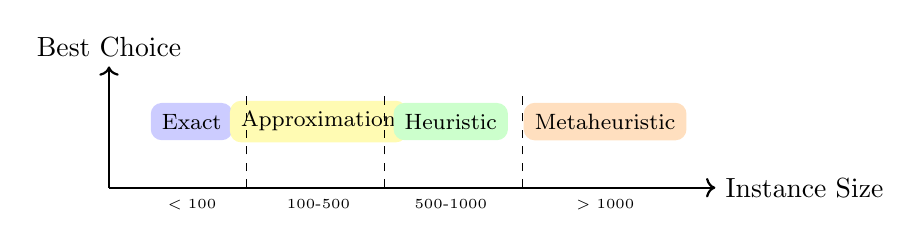
\begin{tikzpicture}[scale=0.7]
\draw[thick, ->] (0,0) -- (11,0) node[right] {Instance Size};
\draw[thick, ->] (0,0) -- (0,2.2) node[above] {Best Choice};
\node[fill=blue!20, rounded corners, inner sep=4pt] at (1.5,1.2) {\footnotesize Exact};
\node[fill=yellow!30, rounded corners, inner sep=4pt] at (3.8,1.2) {\footnotesize Approximation};
\node[fill=green!20, rounded corners, inner sep=4pt] at (6.2,1.2) {\footnotesize Heuristic};
\node[fill=orange!25, rounded corners, inner sep=4pt] at (9,1.2) {\footnotesize Metaheuristic};
\draw[dashed] (2.5,0) -- (2.5,1.8);
\draw[dashed] (5,0) -- (5,1.8);
\draw[dashed] (7.5,0) -- (7.5,1.8);
\node at (1.5,-0.3) {\tiny $<100$};
\node at (3.8,-0.3) {\tiny $100\text{-}500$};
\node at (6.2,-0.3) {\tiny $500\text{-}1000$};
\node at (9,-0.3) {\tiny $>1000$};
\end{tikzpicture}
\end{center}
\end{frame}

% =============================================================================
% SECTION 4: SELECTED ALGORITHMS
% =============================================================================
\section{Implementation Algorithms}

\begin{frame}{Section 4: Algorithms to Implement}
\begin{center}
{\Large\textcolor{primaryblue}{\textbf{Maximum Marginal Return (MMR) and Ant Colony Optimization (ACO)}}}

\vspace{0.3cm}
{\normalsize Detailed algorithms with step-by-step examples}
\end{center}

\vspace{0.2cm}
\begin{columns}[t]
\column{0.48\textwidth}
\begin{block}{\textbf{MMR} -- Greedy Heuristic}
\begin{itemize}
    \item Fast: $O(mn)$ complexity
    \item Deterministic output
    \item Near-optimal ($<$5\% gap)
    \item \textbf{Ideal for real-time systems}
\end{itemize}
\end{block}

\column{0.48\textwidth}
\begin{alertblock}{\textbf{ACO} -- Metaheuristic}
\begin{itemize}
    \item Flexible: $O(I \cdot A \cdot mn)$
    \item Stochastic exploration
    \item Avoids local optima
    \item \textbf{Ideal for large instances}
\end{itemize}
\end{alertblock}
\end{columns}
\end{frame}

\begin{frame}{Why MMR + ACO?}
\begin{columns}[t]
\column{0.48\textwidth}
\begin{block}{\textbf{Maximum Marginal Return (MMR)}}
\textbf{Why selected:}
\begin{itemize}
    \item \textcolor{accentgreen}{$O(mn)$} -- fastest complexity
    \item Simple to implement and verify
    \item Often near-optimal ($<$5\% gap)
    \item Optimal when $p_{ij}$ are uniform
    \item \textbf{Ideal for real-time missile defense}
\end{itemize}

\vspace{0.2cm}
\textbf{Key Formula:}
$$\Delta_{ij} = V_j \cdot q_j \cdot (1 - q_{ij})$$
{\small (Marginal reduction in survival)}
\end{block}

\column{0.48\textwidth}
\begin{alertblock}{\textbf{Ant Colony Optimization (ACO)}}
\textbf{Why selected:}
\begin{itemize}
    \item Avoids premature convergence
    \item Natural exploration/exploitation balance
    \item Pheromone-based learning
    \item \textbf{Effective for large instances ($>$500)}
    \item Elite ant strategy improves quality
\end{itemize}

\vspace{0.2cm}
\textbf{Key Formula:}
$$P_{ij} = \frac{[\tau_{ij}]^\alpha [\eta_{ij}]^\beta}{\sum [\tau]^\alpha [\eta]^\beta}$$
{\small (Transition probability)}
\end{alertblock}
\end{columns}

\vspace{0.3cm}
\begin{exampleblock}{Complementary Approaches}
\textbf{MMR} provides fast initial solution; \textbf{ACO} refines for large-scale instances with multiple ants exploring solution space.
\end{exampleblock}
\end{frame}

% ===== MMR ALGORITHM =====
\begin{frame}{Algorithm 1: Maximum Marginal Return (MMR)}
\begin{block}{Core Idea}
\textbf{Greedy approach:} At each step, assign the weapon-target pair that provides the \textbf{maximum marginal improvement} in expected damage.
\end{block}

\vspace{0.2cm}
\begin{exampleblock}{Key Concepts}
\begin{itemize}
    \item \textbf{Combined Kill Probability:} When multiple weapons assigned to same target:
    $$P_{kill} = 1 - \prod_{i \in S} (1 - p_i)$$
    where $S$ is the set of weapons assigned to that target
    \item \textbf{Expected Value:} $\text{EV} = V_j \times P_{kill,j}$
    \item \textbf{Marginal Return:} $MR_{ij} = V_j \times P'_{kill,j} - V_j \times P_{kill,j}$
\end{itemize}
\end{exampleblock}

\begin{alertblock}{Example: Diminishing Returns}
If W1 ($p=0.7$) and W3 ($p=0.8$) both assigned to T1:
$P_{kill} = 1 - (1-0.7) \times (1-0.8) = 1 - 0.06 = 0.94$
\end{alertblock}
\end{frame}

\begin{frame}[fragile]{MMR Algorithm: Pseudocode}
\begin{algorithm}[H]
\caption{Maximum Marginal Return (MMR) Heuristic for WTA}
\begin{algorithmic}[1]
\State \textbf{Input:} Weapons $W$, Targets $T$, Kill Prob $P$, Threat Values $V$
\State \textbf{Output:} Assignment $A$
\State Initialize $A \gets \emptyset$ (no assignments)
\State Initialize $P_{kill}[j] \gets 0$ for all targets $j$
\While{unassigned weapons remain}
    \State $maxMarginalReturn \gets 0$
    \State $bestPair \gets null$
    \For{each unassigned weapon $i$}
        \For{each target $j$}
            \State Calculate $P'_{kill,j}$ (kill prob with weapon $i$ added)
            \State $MR_{ij} = V_j \times P'_{kill,j} - V_j \times P_{kill,j}$
            \If{$MR_{ij} > maxMarginalReturn$}
                \State $maxMarginalReturn \gets MR_{ij}$, $bestPair \gets (i,j)$
            \EndIf
        \EndFor
    \EndFor
    \State Assign weapon $i$ to target $j$ from $bestPair$
    \State Update $P_{kill,j}$ and mark weapon $i$ as assigned
\EndWhile
\State \Return $A$
\end{algorithmic}
\end{algorithm}
\end{frame}

\begin{frame}{MMR Example: Problem Setup (Naval Air Defense)}
\begin{columns}
\column{0.48\textwidth}
\textbf{Incoming Missiles (Targets):}
\begin{itemize}
    \item \textcolor{red}{T1}: Aircraft Carrier ($V=10$)
    \item \textcolor{orange}{T2}: Destroyer ($V=6$)
    \item \textcolor{yellow!80!black}{T3}: Supply Ship ($V=3$)
\end{itemize}

\vspace{0.3cm}
\textbf{Defensive Weapons:}
\begin{itemize}
    \item W1, W2, W3, W4 (4 interceptors)
\end{itemize}

\vspace{0.3cm}
\textbf{Goal:} Maximize expected damage prevented

\column{0.48\textwidth}
\textbf{Kill Probability Matrix $P_{ij}$:}
\begin{table}[h]
\centering
\small
\begin{tabular}{c|ccc}
     & T1 & T2 & T3 \\ \hline
W1 & 0.7 & 0.8 & 0.9 \\
W2 & 0.6 & 0.7 & 0.8 \\
W3 & 0.8 & 0.6 & 0.7 \\
W4 & 0.5 & 0.9 & 0.6 \\
\end{tabular}
\end{table}

\vspace{0.3cm}
\textbf{Objective Function:}
$$\text{Max } \sum_{j} V_j \times P_{kill,j}$$
\end{columns}
\end{frame}

\begin{frame}{MMR Iteration 1: Calculate Initial Marginal Returns}
\textbf{Algorithm Step:} Calculate marginal return for all weapon-target pairs

\vspace{0.2cm}
\textbf{Formula:} $MR_{ij} = V_j \times P_{ij}$ (since no weapons assigned yet)

\vspace{0.3cm}
\begin{table}[h]
\centering
\begin{tabular}{c|ccc}
\toprule
     & T1 ($V=10$) & T2 ($V=6$) & T3 ($V=3$) \\ \midrule
W1 & $10 \times 0.7 = 7.0$ & $6 \times 0.8 = 4.8$ & $3 \times 0.9 = 2.7$ \\
W2 & $10 \times 0.6 = 6.0$ & $6 \times 0.7 = 4.2$ & $3 \times 0.8 = 2.4$ \\
W3 & $10 \times 0.8 = \textcolor{red}{\textbf{8.0}}$ & $6 \times 0.6 = 3.6$ & $3 \times 0.7 = 2.1$ \\
W4 & $10 \times 0.5 = 5.0$ & $6 \times 0.9 = 5.4$ & $3 \times 0.6 = 1.8$ \\
\bottomrule
\end{tabular}
\end{table}

\begin{alertblock}{MMR Choice}
\textbf{Highest Marginal Return = 8.0} $\Rightarrow$ Assign \textbf{W3 $\rightarrow$ T1}
\end{alertblock}

\textbf{Current State:} T1: $P_{kill} = 0.8$, Expected = 8.0 \quad \textbf{Remaining:} W1, W2, W4
\end{frame}

\begin{frame}{MMR Iteration 2: Recalculate with Diminishing Returns}
\textbf{Algorithm Step:} Update marginal returns accounting for W3 already on T1

\vspace{0.2cm}
\textbf{For T1 (already has W3, $P_{kill} = 0.8$):}
\begin{itemize}
    \item W1: $P'_{kill} = 1-(0.3 \times 0.2) = 0.94$, $MR = 10(0.94-0.8) = 1.4$
    \item W2: $P'_{kill} = 1-(0.4 \times 0.2) = 0.92$, $MR = 10(0.92-0.8) = 1.2$
    \item W4: $P'_{kill} = 1-(0.5 \times 0.2) = 0.90$, $MR = 10(0.90-0.8) = 1.0$
\end{itemize}

\vspace{0.2cm}
\begin{table}[h]
\centering
\begin{tabular}{c|ccc}
\toprule
     & T1 (has W3) & T2 (empty) & T3 (empty) \\ \midrule
W1 & 1.4 & 4.8 & 2.7 \\
W2 & 1.2 & 4.2 & 2.4 \\
W4 & 1.0 & \textcolor{red}{\textbf{5.4}} & 1.8 \\
\bottomrule
\end{tabular}
\end{table}

\begin{alertblock}{MMR Choice}
\textbf{Highest Marginal Return = 5.4} $\Rightarrow$ Assign \textbf{W4 $\rightarrow$ T2}
\end{alertblock}

\textbf{Current State:} T1: 8.0, T2: $6 \times 0.9 = 5.4$ \quad \textbf{Total: 13.4}
\end{frame}

\begin{frame}{MMR Iterations 3 \& 4: Complete Assignment}
\textbf{Iteration 3:} Marginal returns for W1, W2

\begin{table}[h]
\centering
\begin{tabular}{c|ccc}
\toprule
     & T1 (has W3) & T2 (has W4) & T3 (empty) \\ \midrule
W1 & 1.4 & 0.48 & \textcolor{red}{\textbf{2.7}} \\
W2 & 1.2 & 0.42 & 2.4 \\
\bottomrule
\end{tabular}
\end{table}

$\Rightarrow$ Assign \textbf{W1 $\rightarrow$ T3} (MR = 2.7)

\vspace{0.3cm}
\textbf{Iteration 4:} Only W2 remains

\begin{table}[h]
\centering
\begin{tabular}{c|ccc}
\toprule
     & T1 (has W3) & T2 (has W4) & T3 (has W1) \\ \midrule
W2 & \textcolor{red}{\textbf{1.2}} & 0.42 & 0.24 \\
\bottomrule
\end{tabular}
\end{table}

$\Rightarrow$ Assign \textbf{W2 $\rightarrow$ T1} (MR = 1.2)

\begin{exampleblock}{Note: Diminishing Returns}
T3 with W1 has $P_{kill} = 0.9$, so adding W2: $P'_{kill} = 1-(0.2 \times 0.1) = 0.98$, $MR = 3(0.98-0.9) = 0.24$
\end{exampleblock}
\end{frame}

\begin{frame}{MMR: Final Solution}
\begin{center}
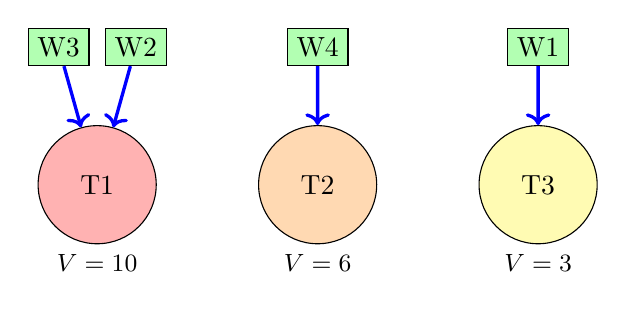
\begin{tikzpicture}[scale=0.7]
% Targets
\node[draw, circle, fill=red!30, minimum size=1.5cm] (T1) at (0,0) {T1};
\node[draw, circle, fill=orange!30, minimum size=1.5cm] (T2) at (4,0) {T2};
\node[draw, circle, fill=yellow!30, minimum size=1.5cm] (T3) at (8,0) {T3};

% Weapons assigned
\node[draw, rectangle, fill=green!30] (W3) at (-0.7,2.5) {W3};
\node[draw, rectangle, fill=green!30] (W2) at (0.7,2.5) {W2};
\node[draw, rectangle, fill=green!30] (W4) at (4,2.5) {W4};
\node[draw, rectangle, fill=green!30] (W1) at (8,2.5) {W1};

% Assignment arrows
\draw[->, very thick, blue] (W3) -- (T1);
\draw[->, very thick, blue] (W2) -- (T1);
\draw[->, very thick, blue] (W4) -- (T2);
\draw[->, very thick, blue] (W1) -- (T3);

% Labels
\node[below] at (T1.south) {\small $V=10$};
\node[below] at (T2.south) {\small $V=6$};
\node[below] at (T3.south) {\small $V=3$};
\end{tikzpicture}
\end{center}

\begin{block}{Final Assignment \& Expected Value}
\begin{itemize}
    \item \textbf{T1 (Aircraft Carrier):} W2, W3 $\rightarrow$ $P_{kill} = 1-(0.4 \times 0.2) = 0.92$, EV = $10 \times 0.92 = 9.2$
    \item \textbf{T2 (Destroyer):} W4 $\rightarrow$ $P_{kill} = 0.9$, EV = $6 \times 0.9 = 5.4$
    \item \textbf{T3 (Supply Ship):} W1 $\rightarrow$ $P_{kill} = 0.9$, EV = $3 \times 0.9 = 2.7$
\end{itemize}
\end{block}

\begin{alertblock}{Total Expected Value (Damage Prevented)}
$9.2 + 5.4 + 2.7 = \mathbf{17.3}$
\end{alertblock}
\end{frame}

\begin{frame}{MMR: Algorithm Analysis}
\begin{columns}[t]
\column{0.48\textwidth}
\begin{block}{Advantages}
\begin{itemize}
    \item \textbf{Fast:} $O(M^2 \cdot N)$ time complexity
    \item \textbf{Simple:} Easy to implement
    \item \textbf{Real-time capable:} Suitable for time-critical defense systems
    \item \textbf{Good results:} Often near-optimal
    \item \textbf{Adaptive:} Considers current state when making decisions
\end{itemize}
\end{block}

\column{0.48\textwidth}
\begin{alertblock}{Disadvantages}
\begin{itemize}
    \item \textbf{No optimality guarantee:} May miss globally optimal solution
    \item \textbf{Greedy nature:} Early decisions can't be reversed
    \item \textbf{Local optimization:} Focuses on immediate best choice
\end{itemize}
\end{alertblock}

\begin{exampleblock}{When to Use MMR}
\begin{itemize}
    \item Speed is critical
    \item Near-optimal is acceptable
    \item Real-time defense systems
    \item Large-scale problems
\end{itemize}
\end{exampleblock}
\end{columns}
\end{frame}

% ===== ACO ALGORITHM =====
\begin{frame}{Algorithm 2: Ant Colony Optimization (ACO)}
\begin{columns}[t]
\column{0.48\textwidth}
\begin{block}{Core Idea}
\textbf{Bio-inspired approach:} Ants deposit pheromones on good paths, guiding future ants toward better solutions.
\end{block}

\vspace{0.2cm}
\begin{center}
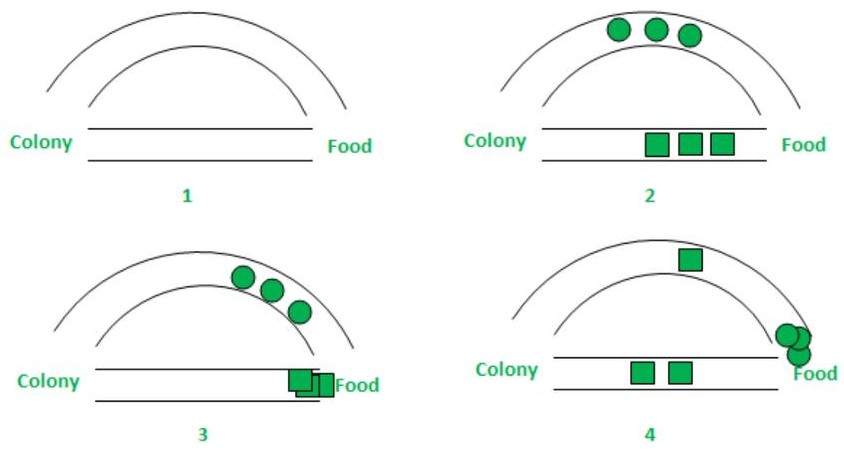
\includegraphics[width=0.95\textwidth]{images/ant_colony_path.jpg}

{\footnotesize Ants find shortest path via pheromone learning}
\end{center}

\column{0.48\textwidth}
\begin{exampleblock}{Key Formulas}
\begin{itemize}
    \item \textbf{Selection:}
    $$P_{ij} = \frac{[\tau_{ij}]^\alpha \cdot [\eta_{ij}]^\beta}{\sum_{l} [\tau_{il}]^\alpha \cdot [\eta_{il}]^\beta}$$
    \item \textbf{Evaporation:} $\tau_{ij} \gets (1-\rho) \cdot \tau_{ij}$
    \item \textbf{Deposit:} $\tau_{ij} \gets \tau_{ij} + Q/F_k$
\end{itemize}
\end{exampleblock}

\begin{alertblock}{Pheromone Influence}
If $(W_1, T_1)$ has $\tau=0.5$ and $(W_1, T_2)$ has $\tau=0.1$: Ant is $5\times$ more likely to choose $T_1$
\end{alertblock}
\end{columns}
\end{frame}

\begin{frame}[fragile]{ACO Algorithm: Pseudocode}
\begin{algorithm}[H]
\caption{Ant Colony Optimization (ACO) Metaheuristic for WTA}
\begin{algorithmic}[1]
\State Initialize pheromone matrix $\tau_{ij} \gets \tau_0$ for all $(i,j)$
\State Set parameters: $\alpha, \beta, \rho, Q, n_{ants}, n_{iter}$
\For{iteration $= 1$ to $n_{iter}$}
    \For{ant $k = 1$ to $n_{ants}$}
        \State Initialize solution $S_k \gets \emptyset$
        \For{weapon $i = 1$ to $m$}
            \State Calculate probability for each available target $j$:
            \State \quad $p_{ij}^k = \frac{[\tau_{ij}]^\alpha \cdot [\eta_{ij}]^\beta}{\sum_{l \in \text{available}} [\tau_{il}]^\alpha \cdot [\eta_{il}]^\beta}$
            \State \quad where $\eta_{ij} = P_{ij} \times V_j$ (heuristic information)
            \State Select target $j$ using roulette wheel selection
            \State Add assignment $(i,j)$ to $S_k$
        \EndFor
        \State Calculate fitness $F_k = \sum_{(i,j) \in S_k} P_{ij} \times V_j$
    \EndFor
    \State \textbf{Pheromone Update:}
    \State \quad Evaporation: $\tau_{ij} \gets (1-\rho) \cdot \tau_{ij}$ for all $(i,j)$
    \State \quad Deposit: $\tau_{ij} \gets \tau_{ij} + \sum_{k: (i,j) \in S_k} \frac{Q}{F_k}$
\EndFor
\State \Return Best solution found
\end{algorithmic}
\end{algorithm}
\end{frame}

\begin{frame}{ACO Example: Problem Setup}
\textbf{3 Weapons, 3 Targets}

\vspace{0.2cm}
\begin{columns}
\column{0.48\textwidth}
\textbf{Kill Probability Matrix ($P_{ij}$):}
\begin{center}
\begin{tabular}{c|ccc}
\toprule
& $T_1$ & $T_2$ & $T_3$ \\
\midrule
$W_1$ & 0.7 & 0.5 & 0.4 \\
$W_2$ & 0.6 & 0.8 & 0.5 \\
$W_3$ & 0.5 & 0.6 & 0.9 \\
\bottomrule
\end{tabular}
\end{center}

\vspace{0.3cm}
\textbf{Target Values:}
\begin{itemize}
    \item $V(T_1) = 100$ (high-value)
    \item $V(T_2) = 80$ (medium-value)
    \item $V(T_3) = 60$ (lower-value)
\end{itemize}

\column{0.48\textwidth}
\textbf{ACO Parameters:}
\begin{center}
\begin{tabular}{ll}
\toprule
\textbf{Parameter} & \textbf{Value} \\
\midrule
Number of ants ($n_{ants}$) & 5 \\
Number of iterations ($n_{iter}$) & 3 \\
Pheromone importance ($\alpha$) & 1 \\
Heuristic importance ($\beta$) & 2 \\
Evaporation rate ($\rho$) & 0.5 \\
Pheromone constant ($Q$) & 1 \\
Initial pheromone ($\tau_0$) & 0.1 \\
\bottomrule
\end{tabular}
\end{center}
\end{columns}
\end{frame}

\begin{frame}{ACO: Heuristic Matrix Initialization}
\textbf{Heuristic Information:} $\eta_{ij} = P_{ij} \times V_j$

\vspace{0.3cm}
\begin{table}[h]
\centering
\begin{tabular}{c|ccc}
\toprule
& $T_1$ ($V=100$) & $T_2$ ($V=80$) & $T_3$ ($V=60$) \\
\midrule
$W_1$ & $0.7 \times 100 = 70$ & $0.5 \times 80 = 40$ & $0.4 \times 60 = 24$ \\
$W_2$ & $0.6 \times 100 = 60$ & $0.8 \times 80 = 64$ & $0.5 \times 60 = 30$ \\
$W_3$ & $0.5 \times 100 = 50$ & $0.6 \times 80 = 48$ & $0.9 \times 60 = 54$ \\
\bottomrule
\end{tabular}
\end{table}

\vspace{0.3cm}
\textbf{Initial Pheromone Matrix:} All entries $= \tau_0 = 0.1$

\begin{exampleblock}{Interpretation}
Higher $\eta_{ij}$ values indicate more attractive weapon-target assignments based on \textbf{expected damage}.
\end{exampleblock}
\end{frame}

\begin{frame}{ACO Iteration 1: Ant 1 Assigns $W_1$}
\textbf{Available targets:} $\{T_1, T_2, T_3\}$

\vspace{0.2cm}
\textbf{Calculate attractiveness:} $[\tau_{ij}]^\alpha \cdot [\eta_{ij}]^\beta$ with $\alpha=1$, $\beta=2$

\begin{align*}
\text{For } T_1: & \quad (0.1)^1 \times (70)^2 = 0.1 \times 4900 = 490 \\
\text{For } T_2: & \quad (0.1)^1 \times (40)^2 = 0.1 \times 1600 = 160 \\
\text{For } T_3: & \quad (0.1)^1 \times (24)^2 = 0.1 \times 576 = 57.6 \\
\text{Sum } \Sigma: & \quad 707.6
\end{align*}

\textbf{Selection Probabilities:}
\begin{itemize}
    \item $P(T_1) = 490/707.6 = \textcolor{red}{\textbf{69.2\%}}$
    \item $P(T_2) = 160/707.6 = 22.6\%$
    \item $P(T_3) = 57.6/707.6 = 8.1\%$
\end{itemize}

\begin{alertblock}{Selection (Roulette Wheel)}
$W_1 \to T_1$ (highest probability selected)
\end{alertblock}
\end{frame}

\begin{frame}{ACO Iteration 1: Ant 1 Completes Solution}
\textbf{Assigning $W_2$:} Available targets $\{T_2, T_3\}$ (T1 taken)

\begin{align*}
\text{For } T_2: & \quad (0.1)^1 \times (64)^2 = 409.6 \quad \Rightarrow P = 82.0\% \\
\text{For } T_3: & \quad (0.1)^1 \times (30)^2 = 90 \quad \Rightarrow P = 18.0\%
\end{align*}
$\Rightarrow W_2 \to T_2$

\vspace{0.3cm}
\textbf{Assigning $W_3$:} Only $T_3$ remains $\Rightarrow W_3 \to T_3$

\vspace{0.3cm}
\begin{exampleblock}{Ant 1 Solution \& Fitness}
\begin{center}
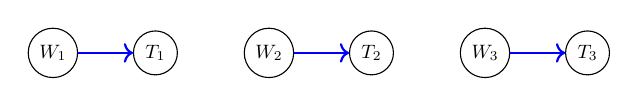
\begin{tikzpicture}[node distance=1cm, scale=0.7, transform shape]
\node[circle, draw] (w1) {$W_1$};
\node[circle, draw, right=of w1] (t1) {$T_1$};
\draw[->, thick, blue] (w1) -- (t1);
\node[circle, draw, right=1.2cm of t1] (w2) {$W_2$};
\node[circle, draw, right=of w2] (t2) {$T_2$};
\draw[->, thick, blue] (w2) -- (t2);
\node[circle, draw, right=1.2cm of t2] (w3) {$W_3$};
\node[circle, draw, right=of w3] (t3) {$T_3$};
\draw[->, thick, blue] (w3) -- (t3);
\end{tikzpicture}
\end{center}
$F_1 = 100 \times 0.7 + 80 \times 0.8 + 60 \times 0.9 = 70 + 64 + 54 = \mathbf{188}$
\end{exampleblock}
\end{frame}

\begin{frame}{ACO Iteration 1: All Ants Complete}
\textbf{All 5 ants construct solutions using probabilistic selection:}

\vspace{0.3cm}
\begin{center}
\begin{tabular}{cllc}
\toprule
\textbf{Ant} & \textbf{Solution} & \textbf{Fitness} \\
\midrule
1 & $W_1\to T_1, W_2\to T_2, W_3\to T_3$ & \textcolor{accentgreen}{\textbf{188}} \\
2 & $W_1\to T_2, W_2\to T_1, W_3\to T_3$ & 154 \\
3 & $W_1\to T_1, W_2\to T_3, W_3\to T_2$ & 148 \\
4 & $W_1\to T_1, W_2\to T_2, W_3\to T_3$ & \textcolor{accentgreen}{\textbf{188}} \\
5 & $W_1\to T_3, W_2\to T_2, W_3\to T_1$ & 138 \\
\bottomrule
\end{tabular}
\end{center}

\vspace{0.3cm}
\textbf{Best solutions:} Ant 1 and Ant 4 (Fitness = 188)

\vspace{0.3cm}
\begin{alertblock}{Key Insight}
Different ants explore different solutions due to \textbf{probabilistic selection}, allowing exploration of solution space!
\end{alertblock}
\end{frame}

\begin{frame}{ACO: Pheromone Update}
\begin{columns}[t]
\column{0.48\textwidth}
\begin{block}{Step 1: Evaporation ($\rho = 0.5$)}
$$\tau_{ij}^{new} = (1-\rho) \times \tau_{ij}^{old}$$

All pheromones: $0.1 \to 0.05$

\begin{center}
\small
\begin{tabular}{c|ccc}
\toprule
& $T_1$ & $T_2$ & $T_3$ \\
\midrule
$W_1$ & 0.05 & 0.05 & 0.05 \\
$W_2$ & 0.05 & 0.05 & 0.05 \\
$W_3$ & 0.05 & 0.05 & 0.05 \\
\bottomrule
\end{tabular}
\end{center}
\end{block}

\column{0.48\textwidth}
\begin{alertblock}{Step 2: Deposit ($\Delta\tau = Q/F_k$)}
Each ant deposits on its path:
\begin{itemize}
    \item Ant 1: $\Delta\tau = 1/188 = 0.0053$
    \item Ant 2: $\Delta\tau = 1/154 = 0.0065$
    \item Ant 3: $\Delta\tau = 1/148 = 0.0068$
    \item Ant 4: $\Delta\tau = 1/188 = 0.0053$
    \item Ant 5: $\Delta\tau = 1/138 = 0.0072$
\end{itemize}
\end{alertblock}
\end{columns}

\vspace{0.3cm}
\begin{columns}[t]
\column{0.48\textwidth}
\begin{block}{Example: $(W_1, T_1)$ Calculation}
\begin{itemize}
    \item After evaporation: 0.05
    \item Ant 1 deposits: +0.0053
    \item Ant 3 deposits: +0.0068
    \item Ant 4 deposits: +0.0053
    \item \textbf{Total:} $= \mathbf{0.0674}$
\end{itemize}
\end{block}

\column{0.48\textwidth}
\begin{exampleblock}{Updated Pheromone Matrix}
\centering
\small
\begin{tabular}{c|ccc}
\toprule
& $T_1$ & $T_2$ & $T_3$ \\
\midrule
$W_1$ & \textcolor{accentgreen}{0.0674} & 0.0565 & 0.0572 \\
$W_2$ & 0.0565 & \textcolor{accentgreen}{0.0691} & 0.0568 \\
$W_3$ & 0.0572 & 0.0568 & \textcolor{accentgreen}{0.0693} \\
\bottomrule
\end{tabular}

\vspace{0.2cm}
{\footnotesize Best paths have higher pheromones!}
\end{exampleblock}
\end{columns}
\end{frame}

\begin{frame}{ACO: Convergence After Multiple Iterations}
\textbf{Process repeats:}
\begin{enumerate}
    \item Ants construct solutions using \textbf{updated pheromones}
    \item Now more likely to choose high-pheromone paths
    \item Good solutions reinforced, bad solutions fade
\end{enumerate}

\vspace{0.3cm}
\textbf{After 3 iterations:}
\begin{itemize}
    \item Pheromones converge on optimal assignment
    \item $(W_1,T_1)$, $(W_2,T_2)$, $(W_3,T_3)$ have much higher pheromones
    \item Most ants select this solution
\end{itemize}

\vspace{0.3cm}
\begin{alertblock}{Final Best Solution}
\begin{center}
\fcolorbox{blue}{blue!10}{$W_1 \to T_1, \quad W_2 \to T_2, \quad W_3 \to T_3$}

\vspace{0.2cm}
\textbf{Fitness = 188} (Maximum possible for this instance!)
\end{center}
\end{alertblock}
\end{frame}

\begin{frame}{ACO: Algorithm Analysis}
\begin{columns}[t]
\column{0.48\textwidth}
\begin{block}{Advantages}
\begin{itemize}
    \item \textbf{Time complexity:} $O(n_{iter} \times n_{ants} \times n^2)$
    \item \textbf{Handles large-scale:} Effective for many weapons/targets
    \item \textbf{Near-optimal:} Finds high-quality solutions without exhaustive search
    \item \textbf{Parallelizable:} Multiple ants work independently
    \item \textbf{Adaptive:} Learns good assignments through pheromone trails
    \item \textbf{Robust:} Avoids local optima via probabilistic exploration
\end{itemize}
\end{block}

\column{0.48\textwidth}
\begin{alertblock}{Disadvantages}
\begin{itemize}
    \item \textbf{Parameter tuning:} Requires careful selection of $\alpha, \beta, \rho, Q$
    \item \textbf{Slower than greedy:} Multiple iterations needed
    \item \textbf{Stochastic:} Different runs may yield different results
\end{itemize}
\end{alertblock}

\begin{exampleblock}{When to Use ACO}
\begin{itemize}
    \item Large-scale instances ($>$500)
    \item Time permits iterations
    \item High solution quality needed
    \item Escaping local optima critical
\end{itemize}
\end{exampleblock}
\end{columns}
\end{frame}

% =============================================================================
% SECTION 5: EXPERIMENTAL DESIGN
% =============================================================================
\section{Experimental Design}

\begin{frame}{Section 5: Experimental Design}
\begin{center}
{\Large\textcolor{primaryblue}{\textbf{How We Will Evaluate Our Implementations}}}

\vspace{0.5cm}
{\normalsize Comprehensive experimental methodology for algorithm comparison}
\end{center}

\vspace{0.3cm}
\begin{columns}[t]
\column{0.32\textwidth}
\begin{block}{Algorithms}
\begin{itemize}
    \item MMR (Greedy)
    \item ACO (Meta)
    \item B\&B (Exact)
\end{itemize}
\end{block}

\column{0.32\textwidth}
\begin{alertblock}{Instances}
\begin{itemize}
    \item 5 size categories
    \item 30 instances each
    \item 150 total tests
\end{itemize}
\end{alertblock}

\column{0.32\textwidth}
\begin{exampleblock}{Metrics}
\begin{itemize}
    \item Quality (gap)
    \item Runtime
    \item Scalability
\end{itemize}
\end{exampleblock}
\end{columns}
\end{frame}

\begin{frame}{Algorithm Comparison Overview}
\begin{block}{Three Algorithmic Approaches}
We implement and compare three fundamentally different approaches to the WTA problem:
\end{block}

\vspace{0.2cm}
\begin{table}[h]
\centering
\begin{tabular}{lccc}
\toprule
\textbf{Algorithm} & \textbf{Type} & \textbf{Complexity} & \textbf{Characteristics} \\
\midrule
MMR & Greedy heuristic & $O(W^2 \cdot T)$ & Fast, deterministic \\
ACO & Metaheuristic & $O(k \cdot A \cdot W \cdot T)$ & Good quality, flexible \\
B\&B & Exact & $O(T^W)$ worst-case & \textcolor{accentgreen}{Optimal} but slow \\
\bottomrule
\end{tabular}
\end{table}

\vspace{0.3cm}
\begin{exampleblock}{Expected Tradeoffs}
\begin{itemize}
    \item \textbf{MMR:} Real-time applications, potentially lower quality but fastest execution
    \item \textbf{ACO:} Balance between quality and time; suitable for medium-large instances
    \item \textbf{B\&B:} Optimal solutions with proof; limited to small instances due to exponential growth
\end{itemize}
\end{exampleblock}
\end{frame}

\begin{frame}{Benchmark Instances: Test Problem Sizes}
\begin{block}{Five Categories of Problem Complexity}
We test across a range of instance sizes to evaluate scalability.
\end{block}

\vspace{0.2cm}
\begin{table}[h]
\centering
\begin{tabular}{lcccc}
\toprule
\textbf{Category} & \textbf{Weapons} & \textbf{Targets} & \textbf{Variables ($W \times T$)} & \textbf{Instances} \\
\midrule
Small & 5 & 5 & 25 & 30 \\
Small-Medium & 10 & 10 & 100 & 30 \\
Medium & 20 & 20 & 400 & 30 \\
Medium-Large & 50 & 50 & 2,500 & 30 \\
Large & 100 & 100 & 10,000 & 30 \\
\bottomrule
\end{tabular}
\end{table}

\begin{alertblock}{Total: 150 Benchmark Instances}
Each category has 30 randomly generated instances for statistical significance.
\end{alertblock}
\end{frame}

\begin{frame}{Instance Generation Protocol}
\begin{columns}[t]
\column{0.48\textwidth}
\begin{block}{Random Parameter Generation}
\textbf{Target Values:}
$$v_j \sim \text{Uniform}(50, 100)$$
{\small Higher values = more important targets}

\vspace{0.2cm}
\textbf{Kill Probabilities:}
$$p_{ij} \sim \text{Uniform}(0.3, 0.9)$$
{\small Realistic range for weapon effectiveness}

\vspace{0.2cm}
\textbf{Weapon Ammunition:}
$$\sum_{i} \mu_i = 2 \times \text{num\_weapons}$$
{\small Total ammo = twice the weapon count}
\end{block}

\column{0.48\textwidth}
\begin{exampleblock}{Storage Format}
\textbf{CSV Format:}
\begin{itemize}
    \item \texttt{instance\_id}: Unique identifier
    \item \texttt{num\_weapons}: $W$ value
    \item \texttt{num\_targets}: $T$ value
    \item \texttt{values}: Comma-separated $v_j$
    \item \texttt{probabilities}: $W \times T$ matrix
    \item \texttt{ammo}: Per-weapon limits
\end{itemize}

\vspace{0.2cm}
\textbf{Reproducibility:}
\begin{itemize}
    \item Fixed random seeds
    \item Stored instance files
\end{itemize}
\end{exampleblock}
\end{columns}
\end{frame}

\begin{frame}{Algorithm Parameter Settings}
\begin{block}{Configuration for Fair Comparison}
All parameters are fixed across all instances to ensure fair comparison.
\end{block}

\vspace{0.3cm}
\begin{table}[h]
\centering
\begin{tabular}{lll}
\toprule
\textbf{Algorithm} & \textbf{Parameters} & \textbf{Rationale} \\
\midrule
\textbf{MMR} & Deterministic (no tuning needed) & Greedy nature requires no parameters \\
\addlinespace
\textbf{ACO} & $\alpha=1.0$ (pheromone weight) & Standard ACO settings from literature \\
             & $\beta=2.0$ (heuristic weight) & Emphasizes problem-specific info \\
             & $\rho=0.1$ (evaporation rate) & Slow evaporation for exploration \\
             & max\_iter $= 1000$ & Sufficient for convergence \\
             & $n_{ants} = 20$ & Balance quality/speed \\
\addlinespace
\textbf{B\&B} & Time limit: 3600s (1 hour) & Practical timeout for experiments \\
              & MIP gap: 0.01\% & Near-optimal termination \\
\bottomrule
\end{tabular}
\end{table}

\begin{alertblock}{Parameter Range Experimentation}
We will test a range of parameter values ($\alpha$, $\beta$, $\rho$, iterations, ants) to analyze sensitivity and optimize performance across different instance sizes.
\end{alertblock}
\end{frame}

\begin{frame}{Performance Metrics: Solution Quality}
\begin{columns}[t]
\column{0.48\textwidth}
\begin{block}{Objective Function Value}
\textbf{Minimize} expected survival value:
$$f(x) = \sum_{j=1}^{n} v_j \prod_{i=1}^{m} (1-p_{ij})^{x_{ij}}$$

Lower $f(x)$ = better solution (more damage inflicted)
\end{block}

\begin{alertblock}{Optimality Gap}
\textbf{Definition:}
$$\text{Gap} = \frac{f_{\text{alg}} - f_{\text{opt}}}{f_{\text{opt}}} \times 100\%$$

\textbf{Interpretation:}
\begin{itemize}
    \item Gap = 0\% means optimal
    \item Gap = 5\% means 5\% worse than optimal
    \item B\&B provides $f_{\text{opt}}$ baseline
\end{itemize}
\end{alertblock}

\column{0.48\textwidth}
\begin{exampleblock}{Quality Comparisons}
\textbf{Primary Questions:}
\begin{enumerate}
    \item How close is MMR to optimal?
    \item Does ACO improve over MMR?
    \item At what size does B\&B timeout?
\end{enumerate}

\vspace{0.2cm}
\textbf{Expected Results:}
\begin{itemize}
    \item MMR: 3-8\% gap
    \item ACO: 1-5\% gap
    \item B\&B: 0\% gap (when terminates)
\end{itemize}
\end{exampleblock}
\end{columns}
\end{frame}

\begin{frame}{Performance Metrics: Computational Efficiency}
\begin{columns}[t]
\column{0.48\textwidth}
\begin{block}{Runtime Metrics}
\textbf{Primary:}
\begin{itemize}
    \item Wall-clock time (seconds)
    \item CPU time (for accuracy)
\end{itemize}

\vspace{0.2cm}
\textbf{Secondary:}
\begin{itemize}
    \item ACO: Iterations to convergence
    \item B\&B: Nodes explored
    \item B\&B: Timeout count
\end{itemize}
\end{block}

\begin{alertblock}{Scalability Limits}
\begin{tabular}{lc}
\toprule
\textbf{Algorithm} & \textbf{Expected Limit} \\
\midrule
MMR & $\sim$1000$\times$1000 \\
ACO & $\sim$500$\times$500 \\
B\&B & $\sim$50$\times$50 \\
\bottomrule
\end{tabular}
\end{alertblock}

\column{0.48\textwidth}
\begin{exampleblock}{Statistical Analysis}
\textbf{Summary Statistics:}
\begin{itemize}
    \item Mean, median, std deviation
    \item Min/max values
    \item Quartiles for box plots
\end{itemize}

\vspace{0.2cm}
\textbf{Significance Testing:}
\begin{itemize}
    \item Wilcoxon signed-rank test
    \item Pairwise comparisons (MMR vs ACO, ACO vs B\&B)
    \item $p < 0.05$ for significance
\end{itemize}

\vspace{0.2cm}
\textbf{Over 30 instances per category:}

Ensures statistical validity
\end{exampleblock}
\end{columns}
\end{frame}

\begin{frame}{Implementation Pipeline}
\begin{columns}[t]
\column{0.32\textwidth}
\begin{block}{Phase 1: Core}
\textbf{Implementation}
\begin{enumerate}
    \item Implement MMR greedy heuristic
    \item Implement ACO metaheuristic
    \item Implement B\&B exact algorithm
    \item Unit tests for correctness
\end{enumerate}
\end{block}

\column{0.32\textwidth}
\begin{alertblock}{Phase 2: Experiments}
\textbf{Experimentation}
\begin{enumerate}
    \item Generate 150 benchmark instances (CSV)
    \item Execute all algorithms
    \item Log: instance\_id, algorithm, objective, runtime, gap
    \item Handle timeouts
\end{enumerate}
\end{alertblock}

\column{0.32\textwidth}
\begin{exampleblock}{Phase 3: Analysis}
\textbf{Visualization}
\begin{enumerate}
    \item Compute summary statistics
    \item Create 6 comparison plots
    \item Statistical significance tests
    \item Final report
\end{enumerate}
\end{exampleblock}
\end{columns}

\vspace{0.3cm}
\begin{center}
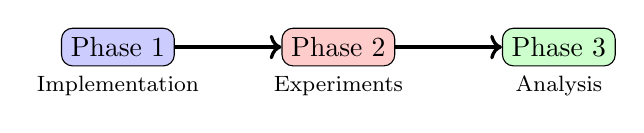
\begin{tikzpicture}[scale=0.7]
\node[draw, rounded corners, fill=blue!20] (p1) at (0,0) {Phase 1};
\node[draw, rounded corners, fill=red!20] (p2) at (4,0) {Phase 2};
\node[draw, rounded corners, fill=green!20] (p3) at (8,0) {Phase 3};
\draw[->, very thick] (p1) -- (p2);
\draw[->, very thick] (p2) -- (p3);
\node at (0,-0.7) {\footnotesize Implementation};
\node at (4,-0.7) {\footnotesize Experiments};
\node at (8,-0.7) {\footnotesize Analysis};
\end{tikzpicture}
\end{center}
\end{frame}

\begin{frame}{Tools and Libraries}
\begin{columns}[t]
\column{0.48\textwidth}
\begin{block}{Programming Environment}
\textbf{Language:} Python 3.11

\vspace{0.2cm}
\textbf{Core Libraries:}
\begin{itemize}
    \item \texttt{numpy}: Numerical operations, matrix manipulation
    \item \texttt{pandas}: Data management, CSV I/O, result aggregation
    \item \texttt{gurobipy}: MILP solver for B\&B exact method
\end{itemize}

\vspace{0.2cm}
\textbf{Visualization:}
\begin{itemize}
    \item \texttt{matplotlib}: Publication-quality plots
    \item \texttt{seaborn}: Statistical visualizations
\end{itemize}
\end{block}

\column{0.48\textwidth}
\begin{exampleblock}{Analysis Libraries}
\textbf{Statistics:}
\begin{itemize}
    \item \texttt{scipy.stats}: Wilcoxon test, normality tests
    \item \texttt{statsmodels}: Advanced statistical analysis
\end{itemize}

\vspace{0.3cm}
\textbf{Output Deliverables:}
\begin{itemize}
    \item Results CSV with all metrics
    \item 6 comparison plots (quality, time, scalability, gaps)
    \item Statistical significance table
    \item Algorithm source code
\end{itemize}
\end{exampleblock}
\end{columns}
\end{frame}

\begin{frame}{Visualization Plan}
\textbf{Six Plots to Generate for Final Analysis:}

\vspace{0.2cm}
\begin{columns}[t]
\column{0.48\textwidth}
\begin{block}{Quality Analysis}
\begin{enumerate}
    \item \textbf{Box Plot:} Objective value distribution by algorithm per problem size
    \item \textbf{Line Plot:} Mean solution quality vs. problem size
    \item \textbf{Gap Chart:} Optimality gap comparison across algorithms
\end{enumerate}
\end{block}

\column{0.48\textwidth}
\begin{alertblock}{Performance Analysis}
\begin{enumerate}
    \setcounter{enumi}{3}
    \item \textbf{Bar Chart:} Average runtime comparison
    \item \textbf{Log-Log Plot:} Scalability curves (runtime vs. size)
    \item \textbf{Stats Table:} Wilcoxon test p-values (pairwise)
\end{enumerate}
\end{alertblock}
\end{columns}

\vspace{0.3cm}
\begin{center}
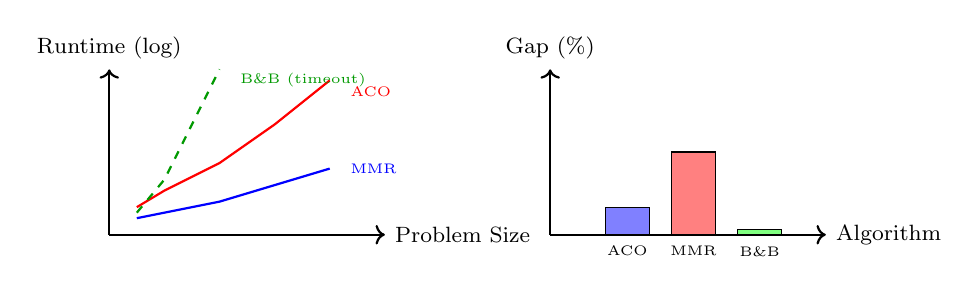
\begin{tikzpicture}[scale=0.7]
% Sample visualization sketch
\draw[thick, ->] (0,0) -- (5,0) node[right] {\footnotesize Problem Size};
\draw[thick, ->] (0,0) -- (0,3) node[above] {\footnotesize Runtime (log)};
\draw[blue, thick] (0.5,0.3) -- (1,0.4) -- (2,0.6) -- (3,0.9) -- (4,1.2);
\draw[red, thick] (0.5,0.5) -- (1,0.8) -- (2,1.3) -- (3,2) -- (4,2.8);
\draw[green!60!black, thick, dashed] (0.5,0.4) -- (1,1) -- (1.5,2) -- (2,3);
\node[blue, right] at (4.2,1.2) {\tiny MMR};
\node[red, right] at (4.2,2.6) {\tiny ACO};
\node[green!60!black, right] at (2.2,2.8) {\tiny B\&B (timeout)};

% Second plot
\draw[thick, ->] (8,0) -- (13,0) node[right] {\footnotesize Algorithm};
\draw[thick, ->] (8,0) -- (8,3) node[above] {\footnotesize Gap (\%)};
\draw[fill=blue!50] (9,0) rectangle (9.8,0.5);
\draw[fill=red!50] (10.2,0) rectangle (11,1.5);
\draw[fill=green!50] (11.4,0) rectangle (12.2,0.1);
\node at (9.4,-0.3) {\tiny ACO};
\node at (10.6,-0.3) {\tiny MMR};
\node at (11.8,-0.3) {\tiny B\&B};
\end{tikzpicture}
\end{center}
\end{frame}

% =============================================================================
% SECTION 6: APPLICATIONS
% =============================================================================
\section{Applications}

\begin{frame}{Section 6: Applications}
\begin{center}
{\Large\textcolor{primaryblue}{\textbf{Real-World Applications of WTA}}}

\vspace{0.5cm}
{\normalsize Military and Civilian Uses of Weapon-Target Assignment}
\end{center}

\vspace{0.3cm}
\begin{block}{WTA is not just a military problem -- it's a fundamental optimization problem!}
The WTA framework applies to any situation involving \textbf{limited resources}, \textbf{multiple objectives}, and \textbf{probabilistic outcomes}.
\end{block}
\end{frame}

\begin{frame}{Why is WTA Important?}
\begin{columns}[t]
\column{0.48\textwidth}
\begin{alertblock}{Theoretical Importance}
\begin{itemize}
    \item \textbf{NP-Complete} problem -- fundamental complexity class
    \item Test case for algorithm research
    \item Used in \textbf{Game Theory} and strategic analysis
    \item Drives optimization innovations
    \item Connections to Knapsack, Assignment, Covering problems
\end{itemize}
\end{alertblock}

\column{0.48\textwidth}
\begin{exampleblock}{Practical Importance}
\begin{itemize}
    \item Military + Civilian applications
    \item \textbf{Saves lives} in emergency response
    \item \textbf{Saves resources} through optimal allocation
    \item Real-time decision making under uncertainty
    \item Growing relevance with autonomous systems
\end{itemize}
\end{exampleblock}
\end{columns}
\end{frame}

\begin{frame}{Military Applications: Air Defense Systems}
\begin{block}{Example: US Navy AEGIS System \& Israel's Iron Dome}
Incoming missiles must be intercepted with limited defensive weapons.
\end{block}

\vspace{0.2cm}
\begin{columns}[t]
\column{0.48\textwidth}
\begin{alertblock}{The Challenge}
\begin{itemize}
    \item Enemy missiles incoming -- which interceptor targets which missile?
    \item \textcolor{red}{\textbf{Time constraint:}} Only \textbf{seconds} to decide
    \item \textcolor{red}{\textbf{Resource constraint:}} Limited interceptor missiles
    \item \textcolor{red}{\textbf{Uncertainty:}} Kill probability $< 100\%$
\end{itemize}
\end{alertblock}

\column{0.48\textwidth}
\begin{exampleblock}{WTA Solution}
\begin{itemize}
    \item \textbf{Weapons:} Interceptor missiles
    \item \textbf{Targets:} Incoming threats
    \item \textbf{Objective:} Maximize expected kill probability
    \item \textcolor{accentgreen}{\textbf{Result:}} 90\%+ interception rate (Iron Dome)
\end{itemize}
\end{exampleblock}
\end{columns}

\vspace{0.2cm}
\begin{center}
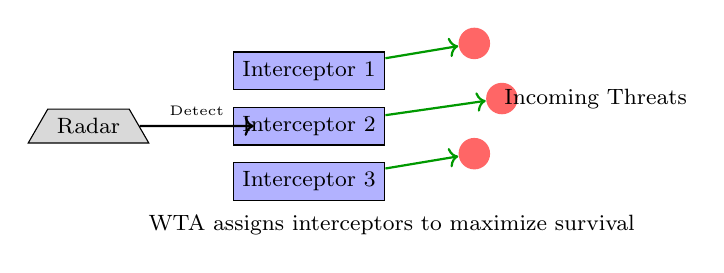
\begin{tikzpicture}[scale=0.7]
% Radar
\node[draw, trapezium, fill=gray!30, minimum width=1cm] (radar) at (-2,0) {\footnotesize Radar};
% Threats
\node[circle, fill=red!60, minimum size=0.4cm] (t1) at (5,1.5) {};
\node[circle, fill=red!60, minimum size=0.4cm] (t2) at (5.5,0.5) {};
\node[circle, fill=red!60, minimum size=0.4cm] (t3) at (5,-0.5) {};
\node at (7.2,0.5) {\footnotesize Incoming Threats};
% Interceptors
\node[draw, rectangle, fill=blue!30] (w1) at (2,1) {\footnotesize Interceptor 1};
\node[draw, rectangle, fill=blue!30] (w2) at (2,0) {\footnotesize Interceptor 2};
\node[draw, rectangle, fill=blue!30] (w3) at (2,-1) {\footnotesize Interceptor 3};
% Assignments
\draw[->, thick, green!60!black] (w1) -- (t1);
\draw[->, thick, green!60!black] (w2) -- (t2);
\draw[->, thick, green!60!black] (w3) -- (t3);
% Label
\draw[->, thick] (radar) -- (1,0) node[midway, above] {\tiny Detect};
\node at (3.5, -1.8) {\footnotesize WTA assigns interceptors to maximize survival};
\end{tikzpicture}
\end{center}
\end{frame}

\begin{frame}{Military Applications: Counter-Drone Systems}
\begin{exampleblock}{Emerging Threat: Drone Swarms}
Modern warfare involves coordinated drone attacks that overwhelm traditional defenses.
\end{exampleblock}

\vspace{0.3cm}
\begin{columns}[t]
\column{0.48\textwidth}
\begin{block}{Available Countermeasures}
\begin{itemize}
    \item \textbf{Electronic Jamming:} Disrupt communications
    \item \textbf{Kinetic Weapons:} Physical destruction
    \item \textbf{Directed Energy:} Lasers, microwave
    \item \textbf{Counter-Drones:} Autonomous interceptors
\end{itemize}
\end{block}

\column{0.48\textwidth}
\begin{alertblock}{WTA for Layered Defense}
\begin{itemize}
    \item Different weapons have different kill probabilities against different drone types
    \item \textbf{Multi-objective:} Cost vs. effectiveness
    \item \textbf{Dynamic:} Real-time reallocation as situation evolves
    \item Hierarchical WTA for layered engagement
\end{itemize}
\end{alertblock}
\end{columns}
\end{frame}

\begin{frame}{Non-Military Applications -- Part 1}
\begin{columns}[t]
\column{0.48\textwidth}
\begin{alertblock}{Emergency Response \& Disaster Management}
\textbf{Scenario:} During disasters -- where to send ambulances, fire trucks?

\vspace{0.2cm}
\textbf{WTA Mapping:}
\begin{itemize}
    \item \textbf{Weapons} = Ambulances, Fire Trucks, Rescue Teams
    \item \textbf{Targets} = Emergency Incidents, Fire Locations, Trapped Victims
    \item \textbf{Kill Probability} = Success rate based on distance, severity
    \item \textbf{Goal} = Minimize casualties, maximize lives saved
\end{itemize}
\end{alertblock}

\column{0.48\textwidth}
\begin{block}{Healthcare -- Hospital ER Triage}
\textbf{Scenario:} Hospital ER -- which doctor treats which patient?

\vspace{0.2cm}
\textbf{WTA Mapping:}
\begin{itemize}
    \item \textbf{Weapons} = Doctors, Nurses, Equipment, Operating Rooms
    \item \textbf{Targets} = Patients with varying conditions
    \item \textbf{Kill Probability} = Treatment success rate
    \item \textbf{Goal} = Maximize expected lives saved (QALY)
\end{itemize}
\end{block}
\end{columns}
\end{frame}

\begin{frame}{Non-Military Applications -- Part 2}
\begin{columns}[t]
\column{0.48\textwidth}
\begin{exampleblock}{Cybersecurity -- Network Defense}
\textbf{Scenario:} Network under attack -- which defense against which threat?

\vspace{0.2cm}
\textbf{WTA Mapping:}
\begin{itemize}
    \item \textbf{Weapons} = Firewalls, IDS/IPS, Honeypots, Analysts
    \item \textbf{Targets} = Intrusions, Malware, DDoS attacks
    \item \textbf{Kill Probability} = Detection/blocking rate
    \item \textbf{Goal} = Block maximum attacks, protect high-value assets
\end{itemize}
\end{exampleblock}

\column{0.48\textwidth}
\begin{alertblock}{Advertising \& Marketing}
\textbf{Scenario:} Which ad to show to which audience?

\vspace{0.2cm}
\textbf{WTA Mapping:}
\begin{itemize}
    \item \textbf{Weapons} = Ad Placements (TV, Facebook, Google)
    \item \textbf{Targets} = Audience Segments (demographics)
    \item \textbf{Kill Probability} = Conversion rate per segment
    \item \textbf{Goal} = Maximum reach/conversion with budget
\end{itemize}
\end{alertblock}
\end{columns}
\end{frame}

\begin{frame}{More Real-World Applications}
\begin{columns}[t]
\column{0.32\textwidth}
\begin{block}{Conservation}
\begin{itemize}
    \item Wildlife protection
    \item Anti-poaching patrol allocation
    \item Nature reserve selection
    \item Species preservation resources
\end{itemize}
\end{block}

\column{0.32\textwidth}
\begin{alertblock}{Search \& Rescue (SAR)}
\begin{itemize}
    \item Lost person search operations
    \item Maritime SAR
    \item Team allocation to sectors
    \item Probabilistic area coverage
\end{itemize}
\end{alertblock}

\column{0.32\textwidth}
\begin{exampleblock}{Transportation \& Logistics}
\begin{itemize}
    \item Vehicle routing
    \item Delivery optimization
    \item Fleet management
    \item Airport gate assignment
\end{itemize}
\end{exampleblock}
\end{columns}

\vspace{0.5cm}
\begin{block}{Common Pattern Across All Applications}
All these problems involve: \textbf{Limited Resources} + \textbf{Multiple Objectives} + \textbf{Probabilistic Outcomes} + \textbf{Value Prioritization}
\end{block}
\end{frame}

\begin{frame}{Computational Challenges in Real Applications}
\begin{columns}[t]
\column{0.48\textwidth}
\begin{block}{Time Constraints Vary by Domain}
\begin{itemize}
    \item \textcolor{red}{\textbf{Missile Defense:}} Only a few \textbf{seconds}!
    \item \textcolor{orange}{\textbf{Emergency Response:}} A few \textbf{minutes}
    \item \textcolor{yellow!80!black}{\textbf{Healthcare Triage:}} \textbf{Hours}
    \item \textcolor{accentgreen}{\textbf{Advertising Planning:}} \textbf{Days to weeks}
\end{itemize}

\vspace{0.3cm}
$\Rightarrow$ \textbf{Different time constraints require different algorithms!}
\end{block}

\column{0.48\textwidth}
\begin{alertblock}{Computational Problems}
\begin{enumerate}
    \item \textbf{NP-Complete:} Finding optimal solution takes exponential time
    \item \textbf{Large Scale:} Thousands of variables possible (100+ weapons $\times$ 100+ targets)
    \item \textbf{Uncertainty:} Must handle probabilistic outcomes
    \item \textbf{Real-time:} Some applications need instant decisions
    \item \textbf{Dynamic:} Situation changes during execution
\end{enumerate}
\end{alertblock}
\end{columns}

\vspace{0.3cm}
\begin{exampleblock}{Solution: Algorithm Selection Based on Time Budget}
\textbf{Real-time (seconds):} Use \textbf{MMR} greedy heuristic \quad
\textbf{Planning (minutes-hours):} Use \textbf{ACO} or \textbf{B\&B}
\end{exampleblock}
\end{frame}

\begin{frame}{Key Takeaways: WTA Applications}
\textbf{Universal Problem:}
\begin{itemize}
    \item WTA is not just for warfare -- used in emergency services, healthcare, advertising, conservation, cybersecurity, transportation
\end{itemize}

\textbf{Computational Challenge:}
\begin{itemize}
    \item NP-Complete problem -- exact solution very difficult for large scale
    \item Different time constraints require different algorithmic approaches
\end{itemize}

\textbf{Real-World Impact:}
\begin{itemize}
    \item \textbf{Saves lives} in missile defense and emergency response
    \item \textbf{Saves money} in resource allocation and advertising
    \item \textbf{Saves time} through automated decision making
\end{itemize}

\textbf{Algorithm Research:}
\begin{itemize}
    \item Drives development of new optimization techniques (metaheuristics, approximation algorithms)
    \item Connections to other NP-hard problems enable knowledge transfer
\end{itemize}
\end{frame}

% =============================================================================
% CONCLUSION & REFERENCES
% =============================================================================
\section{Conclusion}

\begin{frame}{Summary}
\begin{center}
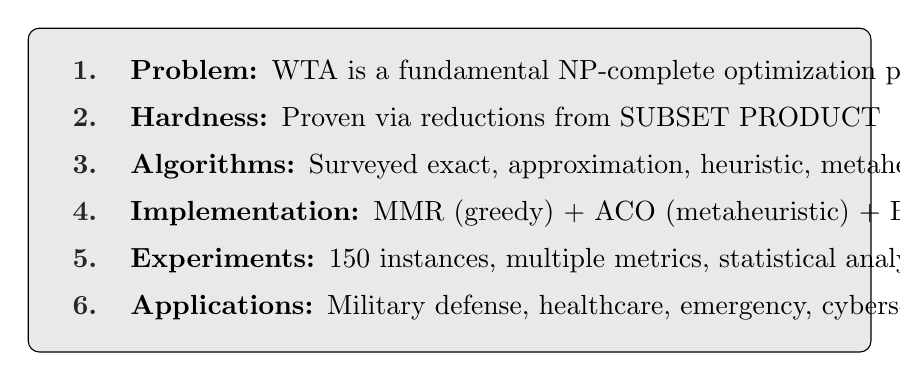
\begin{tikzpicture}[scale=1, transform shape]
\node[draw, rounded corners, fill=primaryblue!10, text width=10cm, align=center, inner sep=10pt] {
\begin{tabular}{cl}
\textcolor{primaryblue}{\textbf{1.}} & \textbf{Problem:} WTA is a fundamental NP-complete optimization problem \\[5pt]
\textcolor{primaryblue}{\textbf{2.}} & \textbf{Hardness:} Proven via reductions from SUBSET PRODUCT \\[5pt]
\textcolor{primaryblue}{\textbf{3.}} & \textbf{Algorithms:} Surveyed exact, approximation, heuristic, metaheuristic \\[5pt]
\textcolor{primaryblue}{\textbf{4.}} & \textbf{Implementation:} MMR (greedy) + ACO (metaheuristic) + B\&B (exact) \\[5pt]
\textcolor{primaryblue}{\textbf{5.}} & \textbf{Experiments:} 150 instances, multiple metrics, statistical analysis \\[5pt]
\textcolor{primaryblue}{\textbf{6.}} & \textbf{Applications:} Military defense, healthcare, emergency, cybersecurity \\
\end{tabular}
};
\end{tikzpicture}
\end{center}

\vspace{0.5cm}
\begin{columns}
\column{0.48\textwidth}
\begin{block}{Next Steps}
\begin{itemize}
    \item Complete Python implementation
    \item Run all benchmark experiments
    \item Generate visualizations \& report
\end{itemize}
\end{block}

\column{0.48\textwidth}
\begin{exampleblock}{Expected Outcomes}
\begin{itemize}
    \item MMR: Fast, $<$5\% gap
    \item ACO: Better quality, slower
    \item B\&B: Optimal for small instances
\end{itemize}
\end{exampleblock}
\end{columns}
\end{frame}

\begin{frame}{References (1/2)}
\begin{columns}[t]
\column{0.48\textwidth}
\scriptsize
\begin{thebibliography}{99}
\bibitem{ahuja2007}
Ahuja, R. K., et al. (2007). \textit{Exact and heuristic algorithms for WTA}. Operations Research.

\bibitem{bertsimas2025}
Bertsimas, D., et al. (2025). \textit{Solving large-scale WTA using branch-price-and-cut}. Naval Research Logistics.

\bibitem{andersen2022}
Andersen, A. C., et al. (2022). \textit{WTA: Exact and approximate algorithms}. Ann. Oper. Res.

\bibitem{camm2002}
Camm, J. D., et al. (2002). \textit{Nature reserve site selection}. Operations Research.

\bibitem{kwon1999}
Kwon, O., et al. (1999). \textit{Lagrangian relaxation approach to targeting}. Naval Research Logistics.

\bibitem{kim2022}
Kim, K., et al. (2022). \textit{WTA model for ground combat using MINLP}. Math. Prob. Eng.
\end{thebibliography}

\column{0.48\textwidth}
\scriptsize
\begin{thebibliography}{99}
\setcounter{enumiv}{6}
\bibitem{hindawi2017}
Li, Y., et al. (2017). \textit{Modified Pareto ACO for bi-objective WTA}. Int. J. Aerospace Eng.

\bibitem{kline2020}
Kline, A. G., et al. (2020). \textit{Heuristic and metaheuristic for static WTA}. J. Global Optim.

\bibitem{intechopen2020}
Sonuc, E., et al. (2020). \textit{Weapon target assignment}. IntechOpen.

\bibitem{xin2018}
Xin, B., et al. (2018). \textit{Marginal-return-based heuristic for sensor-WTA}. IEEE Trans. SMC.
\end{thebibliography}
\end{columns}
\end{frame}

\begin{frame}{References (2/2)}
\begin{columns}[t]
\column{0.48\textwidth}
\scriptsize
\begin{thebibliography}{99}
\setcounter{enumiv}{10}
\bibitem{lee2003}
Lee, Z. J., et al. (2003). \textit{Hybrid ACO-GA for WTA}. IDEAL 2003.

\bibitem{bogdanowicz2013}
Bogdanowicz, Z. R., et al. (2013). \textit{Optimization of weapon-target pairings}. IEEE Trans. Cybernetics.

\bibitem{lee2002}
Lee, Z. J., et al. (2002). \textit{Immunity-based ACO for WTA}. Applied Soft Computing.
\end{thebibliography}

\column{0.48\textwidth}
\scriptsize
\begin{thebibliography}{99}
\setcounter{enumiv}{13}
\bibitem{hu2018}
Hu, X., et al. (2018). \textit{Improved ACO for WTA}. Math. Prob. Eng.

\bibitem{li2017}
Li, Y., et al. (2017). \textit{Modified Pareto ACO for bi-objective WTA}. Int. J. Aerospace Eng.

\bibitem{lloyd1986}
Lloyd, S. P., et al. (1986). \textit{Weapons allocation is NP-complete}. IEEE.
\end{thebibliography}
\end{columns}
\end{frame}

\begin{frame}[plain]
\begin{center}
\vspace{2cm}
{\Huge\textbf{\textcolor{primaryblue}{Thank You!}}}

\vspace{1cm}
{\Large Questions?}

\end{center}
\end{frame}

\end{document}